% ===========================================================
%  Regulación del Alquiler y Dinámica del Mercado Residencial
%  en Barcelona (2000–2025)  ·  Versión 4
%  Estructura guiada por preguntas de investigación
%  Compilar con pdfLaTeX en Overleaf (dos pasadas)
% ===========================================================
\documentclass[10pt,a4paper,twocolumn]{article}

\usepackage[utf8]{inputenc}
\usepackage[T1]{fontenc}
\usepackage[spanish,english]{babel}
\usepackage[top=2.0cm,bottom=2.0cm,left=1.6cm,right=1.6cm,columnsep=0.6cm]{geometry}
\usepackage{microtype}
\usepackage{lmodern}
\usepackage{times}
\usepackage{amsmath,amssymb,amsthm}
\usepackage{bm}
\usepackage{booktabs}
\usepackage{threeparttable}
\usepackage{multirow}
\usepackage{array}
\usepackage{siunitx}
\sisetup{group-separator={.}, group-minimum-digits=4}
\usepackage{graphicx}
\usepackage{subcaption}
\usepackage{float}
\usepackage[dvipsnames]{xcolor}
\usepackage[colorlinks=true,linkcolor=NavyBlue,
            citecolor=NavyBlue,urlcolor=NavyBlue]{hyperref}
\usepackage{natbib}
\usepackage{setspace}
\setstretch{1.05}
\usepackage{parskip}
\setlength{\parskip}{3pt}
\usepackage{titlesec}
\titlespacing*{\section}{0pt}{8pt}{4pt}
\titlespacing*{\subsection}{0pt}{6pt}{2pt}
\titlespacing*{\subsubsection}{0pt}{4pt}{2pt}
\titleformat{\section}{\normalfont\large\bfseries}{\thesection.}{0.5em}{}
\titleformat{\subsection}{\normalfont\normalsize\bfseries}{\thesubsection.}{0.4em}{}
\titleformat{\subsubsection}{\normalfont\small\bfseries\itshape}{\thesubsubsection.}{0.4em}{}
\usepackage{caption}
\captionsetup{font=small,labelfont=bf,skip=4pt}
\usepackage{fancyhdr}
\pagestyle{fancy}
\fancyhf{}
\fancyhead[L]{\small\textit{Soto, Ortiz, Delgado · Regulación del alquiler en Barcelona}}
\fancyhead[R]{\small\textit{2026}}
\fancyfoot[C]{\small\thepage}
\renewcommand{\headrulewidth}{0.4pt}
\usepackage{enumitem}
\setlist[itemize]{itemsep=1pt,topsep=2pt}
\setlist[enumerate]{itemsep=1pt,topsep=2pt}

% --- MEJORAS DE FORMATO PARA COLUMNAS Y FLOTANTES ---
\usepackage{balance} % Para balancear las columnas en la última página
\setlength{\textfloatsep}{12pt plus 2.0pt minus 2.0pt} % Espacio entre imagen y texto
\setlength{\floatsep}{10pt plus 2.0pt minus 2.0pt}     % Espacio entre dos imágenes
\setlength{\intextsep}{10pt plus 2.0pt minus 2.0pt}    % Espacio para [h]
% ----------------------------------------------------

\newcommand{\pval}[1]{$p{=}#1$}
\newcommand{\MAPE}{\text{MAPE}}
\newcommand{\RMSE}{\text{RMSE}}

% ===========================================================
\begin{document}
\selectlanguage{spanish}

\twocolumn[{%
\begin{@twocolumnfalse}
\begin{center}
  {\LARGE\bfseries
   Regulación del Alquiler y Dinámica del Mercado\\[4pt]
   Residencial en Barcelona (2000--2025):\\[4pt]
   Tres Preguntas de Investigación sobre Actividad Contractual,\\[4pt]
   Tensión de Mercado e Impacto de Intervenciones Regulatorias}

  \vspace{8pt}
  {\large Katherine Soto \quad$\cdot$\quad Juan R.\ Ortiz \quad$\cdot$\quad Emilio Delgado}

  \vspace{3pt}
  {\normalsize La Salle -- Universitat Ramon Llull, Barcelona}\\[2pt]
  {\small \href{mailto:katherine.soto@students.salle.url.edu}{\texttt{katherine.soto@students.salle.url.edu}} \quad
          \href{mailto:juanricardo.ortiz@students.salle.url.edu}{\texttt{juanricardo.ortiz@students.salle.url.edu}} \quad
          \href{mailto:emilio.delgado@students.salle.url.edu}{\texttt{emilio.delgado@students.salle.url.edu}}}

  \vspace{3pt}
  {\small Proyecto 2.1  · Máster en Ciencia de Datos · Abril 2026}\\
  {\small GitHub: \url{https://github.com/kateincoding/analisis-regulacion-alquiler-habitual-barcelona}}
\end{center}

\vspace{6pt}

\begin{abstract}
\noindent
Analizamos el mercado de alquiler habitual en Barcelona a lo largo de tres ciclos
regulatorios sucesivos (Ley~11/2020, derogación del Tribunal Constitucional en 2022
y Ley~12/2023) con datos trimestrales de Incasol -- Generalitat de Catalunya
(10 distritos, 2000Q1--2025Q3; 66 barrios, 2014Q1--2025Q3), IPC del INE (base~2025)
y Euríbor del Banco de España. El análisis se organiza en torno a tres preguntas:
cómo se asocia la regulación con la actividad contractual, dónde y cuándo emerge
la tensión de mercado, y qué impacto tienen las intervenciones sobre precio y volumen.
Para responderlas empleamos regresión de panel con efectos fijos ($N{=}2.838$),
clasificación supervisada con ingeniería de características por retardos temporales
y panel logit, y modelos SARIMAX$(1,1,1)(1,0,1)_4$ con análisis de intervención ITS-3.
Con lag features el AUC del Random Forest sube de 0.553 a 0.684. El ITS-3 muestra
que la Ley~12/2023 contrae los contratos de alquiler habitual y eleva el precio real,
consistente con un efecto composición por retirada selectiva de oferta. El análisis
de sustitución sitúa la tasa crítica de migración a temporada en el 20.3\,\%.
\end{abstract}

\vspace{4pt}
\noindent\textbf{Palabras clave:} regulación del alquiler · ITS multi-ruptura · panel efectos
fijos · clasificación supervisada · SHAP · panel logit · zona tensionada · efecto composición · Barcelona.

\vspace{8pt}

\begin{otherlanguage}{english}
\begin{abstract}
\noindent
We analyze the habitual rental market in Barcelona across three successive regulatory
cycles (Law~11/2020, its annulment by the Constitutional Court in 2022, and Law~12/2023)
using quarterly data from Incasol -- Generalitat de Catalunya (10 districts, 2000Q1--2025Q3;
66 neighborhoods, 2014Q1--2025Q3), CPI from INE (base~2025), and Euribor from the Bank
of Spain. The analysis is structured around three questions: how regulation is associated
with contractual activity, where and when market tension emerges, and what impact
interventions have on price and volume. To address them, we employ fixed-effects panel
regression ($N{=}2{,}838$), supervised classification with lagged features and panel logit,
and SARIMAX$(1,1,1)(1,0,1)_4$ models with ITS-3 intervention analysis. Lag features raise
the Random Forest AUC from 0.553 to 0.684. The ITS-3 results show that Law~12/2023
reduces the number of habitual rental contracts and increases real prices, consistent with
a composition effect driven by selective supply withdrawal. Sensitivity analysis places the
critical substitution rate into short-term rentals at 20.3\%.
\end{abstract}
\vspace{4pt}
\noindent\textbf {Keywords:} rent control · interrupted time series · panel data · supervised classification
· SHAP · panel logit · tensioned market zone · composition effect · Barcelona.

\end{otherlanguage}

\vspace{10pt}\hrule\vspace{8pt}
\end{@twocolumnfalse}
}]

% ===========================================================
\section{Introducción}
\label{sec:intro}

La vivienda en alquiler concentra hoy la mayor parte de la presión de asequibilidad
en las grandes ciudades europeas. Barcelona ofrece un caso de estudio con características
difíciles de replicar: en cinco años (2020--2025) transitó por tres regímenes regulatorios
sucesivos, generando una variación institucional exógena densa y temporalmente localizada
que facilita el análisis cuantitativo del impacto regulatorio.

\subsection*{Las tres preguntas que articulan este estudio}

Este estudio se organiza alrededor de tres preguntas 
empíricas sustantivas. Primero, ¿cómo se asocia la secuencia de
cambios regulatorios con la evolución de la actividad contractual, tanto a nivel de
barrio como a nivel de ciudad? Segundo, ¿dónde y cuándo emergen los episodios de
contracción severa del mercado, y qué señales permiten anticiparlos? Tercero,
¿qué impacto cuantificable tienen cada una de las tres intervenciones regulatorias
sobre el precio nominal, el precio real y el volumen de contratos de larga duración?

\subsection*{La lógica contrafactual del diseño}

El instrumento analítico central para las preguntas uno y tres es el modelo de
series temporales interrumpidas con tres rupturas (ITS-3). Este diseño construye
implícitamente un contrafactual: la trayectoria que habrían seguido el precio y el
volumen si las intervenciones regulatorias no hubieran ocurrido, extrapolando la
tendencia estimada en el período pre-intervención. La brecha entre la serie observada
y ese contrafactual modelado es la estimación del efecto regulatorio.

Esta lógica tiene tres supuestos que conviene hacer explícitos. Primero, que la
tendencia pre-intervención habría continuado en ausencia de la regulación (supuesto
de tendencia paralela en el tiempo, no entre unidades). Segundo, que no existe
ningún otro evento simultáneo a la intervención que explique la ruptura de igual
forma (exclusión de confundidores temporales). Tercero, que la regulación afecta
al mercado desde su entrada en vigor legal, y no antes (ausencia de efectos de
anticipación en los datos, aunque los discutimos en la sección~\ref{sec:discusion}).
Cada uno de estos supuestos tiene limitaciones que se documentan en las secciones
de metodología y discusión.

La regresión de panel con efectos fijos responde la primera pregunta desde una
perspectiva diferente: controla por las características no observadas y estables de
cada barrio (localización, densidad, composición sociodemográfica) y estima la
asociación entre-barrio entre los indicadores regulatorios y la actividad contractual.
El panel logit extiende este diseño a la variable dependiente binaria de tensión.

\subsection*{Contribuciones respecto a la literatura}

En el estado del arte se encontraron estos trabajos anteriores para el caso español \citep{garcia2018housing,bosch2021ley11},
este trabajo aporta cuatro elementos. Primero, ingeniería de características temporales
(retardos-1 y retardos-4) que elevan el AUC del clasificador de tensión de 0.553 a 0.684.
Segundo, un panel logit con efectos fijos de barrio que complementa al Random Forest
con coeficientes directamente interpretables en términos de odds ratios. Tercero, un
análisis ITS-3 sobre 30 combinaciones distrito$\times$métrica que documenta la
heterogeneidad geográfica del impacto regulatorio con errores HAC Newey-West.
Cuarto, un análisis formal de sensibilidad al sesgo de sustitución hacia contratos
de temporada que cuantifica la tasa crítica de migración necesaria para que el
efecto negativo sobre volumen sea estadísticamente nulo.

\subsection*{Estructura del artículo}

La Sección~\ref{sec:contexto} describe el contexto regulatorio e institucional.
La Sección~\ref{sec:datos} presenta los datos.
La Sección~\ref{sec:metodos} desarrolla la metodología.
Las Secciones~\ref{sec:rq1}, \ref{sec:rq2} y~\ref{sec:rq3} responden las tres preguntas.
La Sección~\ref{sec:discusion} discute las implicaciones y limitaciones.
La Sección~\ref{sec:conclusiones} cierra con conclusiones.

% ===========================================================
\section{Contexto Regulatorio e Institucional}
\label{sec:contexto}

Comprender el diseño econométrico requiere conocer con precisión la cronología
regulatoria. La Tabla~\ref{tab:cronologia} resume los cinco períodos del análisis.

\begin{table}[!t]
\caption{Períodos regulatorios analizados (2000--2025)}
\label{tab:cronologia}
\centering\small
\begin{tabular}{clp{4.2cm}}
\toprule
Cód. & Fechas & Régimen \\
\midrule
P1 & 2000Q1--2019Q4 & Mercado libre, sin topes de precio \\
P2 & 2020Q1--2020Q3 & Shock COVID ($-22$\,\% contratos interanual) \\
P3 & 2020Q4--2022Q1 & Ley 11/2020: topes catalanes \\
P4 & 2022Q2--2023Q2 & Derogación TC: vacío regulatorio \\
P5 & 2023Q3--2025Q3 & Ley 12/2023: zona tensionada estatal \\
\bottomrule
\end{tabular}
\end{table}

\subsubsection*{Ley 11/2020 (P3, 2020Q4--2022Q1)}

El Parlamento de Catalunya aprobó la Ley 11/2020 de contención de rentas en
septiembre de 2020, con aplicación desde el 22 de octubre de ese año. La ley
fijaba topes a las rentas en los municipios declarados de mercado tensionado,
incluyendo Barcelona y 60 municipios más de la área metropolitana. El tope se
aplicaba sobre el precio del contrato anterior para contratos de renovación,
y sobre el índice de precios de referencia para nuevos contratos. Es importante
señalar que la ley no era retroactiva: los contratos vigentes antes de su entrada
en vigor quedaban excluidos, lo que limita su efecto inmediato al flujo de nuevos
contratos y renovaciones.

\subsubsection*{Derogación del Tribunal Constitucional (P4, 2022Q2--2023Q2)}

En marzo de 2022 el Tribunal Constitucional declaró inconstitucional la Ley~11/2020
por invasión de competencias estatales, con efectos inmediatos desde la publicación
de la sentencia (abril de 2022). El período que sigue, que denominamos vacío
regulatorio, es analíticamente relevante porque elimina los topes sobre contratos
que habrían estado cubiertos bajo la ley catalana. El mercado opera sin restricción
de precios en nuevos contratos durante cinco trimestres, lo que facilita la
comparación directa entre los períodos con y sin regulación.

\subsubsection*{Ley 12/2023 (P5, 2023Q3 en adelante)}

La Ley estatal 12/2023 por el Derecho a la Vivienda establece el mecanismo de
declaración de zonas de mercado residencial tensionado a escala nacional. Barcelona
fue declarada zona tensionada en julio de 2023 (inicio del P5 en nuestro análisis).
La implementación efectiva del control de precios requería la aprobación del índice
de referencia estatal, que no estuvo operativo hasta finales de 2024. Esto implica
que durante una parte del P5 la regulación existía legalmente pero sus mecanismos de
limitación de rentas no eran plenamente aplicables. Esta distinción entre vigencia
legal y aplicación efectiva es relevante para interpretar los coeficientes del ITS-3
en el período P5: recogen el efecto combinado de la señal regulatoria (anuncio y
declaración de zona tensionada) y de la aplicación progresiva de los límites.
La Ley~12/2023 diferencia además entre grandes tenedores (cinco o más inmuebles)
y pequeños propietarios, con restricciones más estrictas para los primeros, lo que
introduce una asimetría de respuesta que los datos agregados no permiten separar.

% ===========================================================
\section{Datos y Preparación}
\label{sec:datos}

\subsection{Fuentes, cobertura y variables}

El análisis integra cuatro fuentes de datos oficiales
\citep{incasol2025,ine2025ipc,bde2025euribor,idescat2025ist}
combinadas mediante union temporal por trimestre:

\begin{enumerate}[leftmargin=*,itemsep=2pt]
  \item \textbf{Contratos de alquiler:}
    \href{https://habitatge.gencat.cat/ca/dades/indicadors_estadistiques/estadistiques_de_construccio_i_mercat_immobiliari/mercat_de_lloguer/lloguers-barcelona-per-districtes-i-barris/}{Incasol -- Generalitat de Catalunya}.
    Distritos: 2000Q1--2025Q3 ($T{=}103$, 10~distritos; base del análisis de
    series temporales). Barrios: 2014Q1--2025Q3 ($T{=}47$, 66~barrios; 7~excluidos
    por mediana inferior a 300 contratos/trimestre; base del
análisis de paneles y clasificación).
  \item \textbf{Índice de Precios de Consumo (IPC) base~2025:}
    \href{https://www.ine.es/jaxiT3/Datos.htm?t=24078}{INE, tabla 24078}.
  \item \textbf{Euríbor 12 meses:}
    \href{https://app.bde.es/bie_www/bie_wwwias/xml/Arranque.html?Idioma=es}{Banco de España, BIE}.
  \item \textbf{Índice Socioeconómico Territorial:}
    \href{https://www.idescat.cat/dades/obertes/ist/}{Idescat},
    usado como proxy de nivel socioeconómico de barrio en la fase exploratoria.
\end{enumerate}

Definimos tres métricas analíticas:
\begin{align}
  \texttt{avg\_rent\_m2}_t &= \frac{\sum_i w_{it} r_{it}}{\sum_i w_{it}}
  \label{eq:nominal}\\
  \texttt{avg\_rent\_m2\_real}_t &= \texttt{avg\_rent\_m2}_t \times \frac{100}{\text{IPC}_t^{(2025)}}
  \label{eq:real}\\
  \texttt{num\_contracts}_t &= \sum_i n_{it}
  \label{eq:vol}
\end{align}
donde $w_{it}$ es el número de contratos del submercado $i$ en el trimestre $t$.
La media ponderada en~\eqref{eq:nominal} evita el sesgo de composición de tamaño
de distrito. El precio real~\eqref{eq:real} está disponible desde 2002Q1.

La Figura~\ref{fig:eda_series} muestra la evolución temporal. La comparación entre
nominal y real revela que el incremento del $+180$\,\% en 20 años es mayoritariamente
inflacionario: en términos reales la variación es del $+14$\,\%.

\begin{figure}[!t]
  \centering
  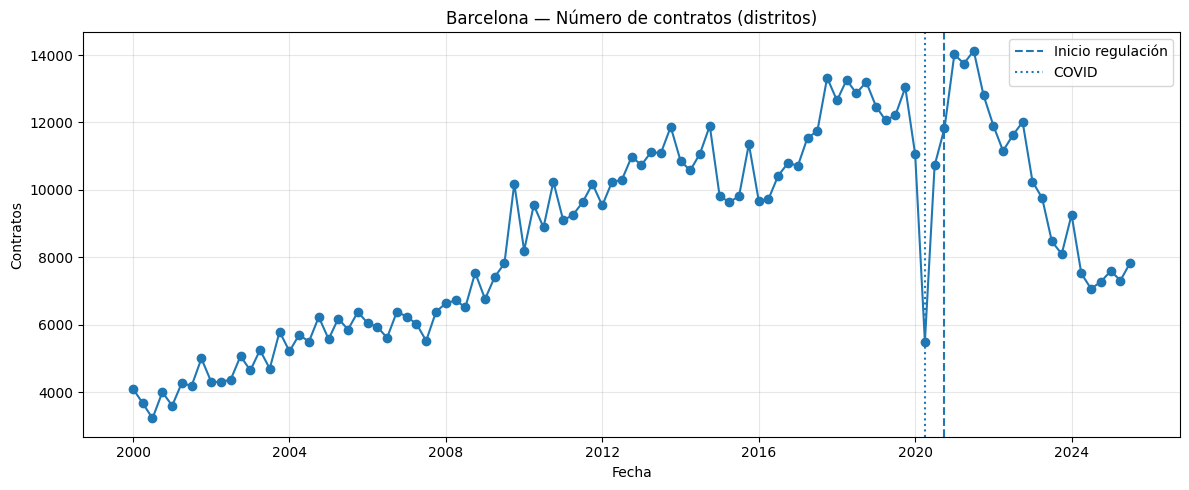
\includegraphics[width=\linewidth]{figures/fig_eda_series.png}
  \caption{Series trimestrales 2000--2025 (Barcelona ciudad). Línea  punteada:
    inicio COVID (2020Q1). Línea discontinua: Ley~11/2020 (2020Q4).
    La divergencia entre precio nominal y precio real ilustra el peso del
    componente inflacionario en el ciclo reciente.}
  \label{fig:eda_series}
\end{figure}

\subsection{Análisis exploratorio y cambio estructural}

La Figura~\ref{fig:eda_5periods} desagrega las distribuciones por período regulatorio.
La Figura~\ref{fig:eda_chow} muestra el test de Chow confirma ruptura estructural en 2020Q4 para precio nominal
($F{=}5.16$, $p{=}0.007$) y contratos ($F{=}101.2$, $p{<}0.001$), pero no para
precio real ($F{=}0.28$, $p{=}0.755$).

\begin{figure}[!t]
  \centering
  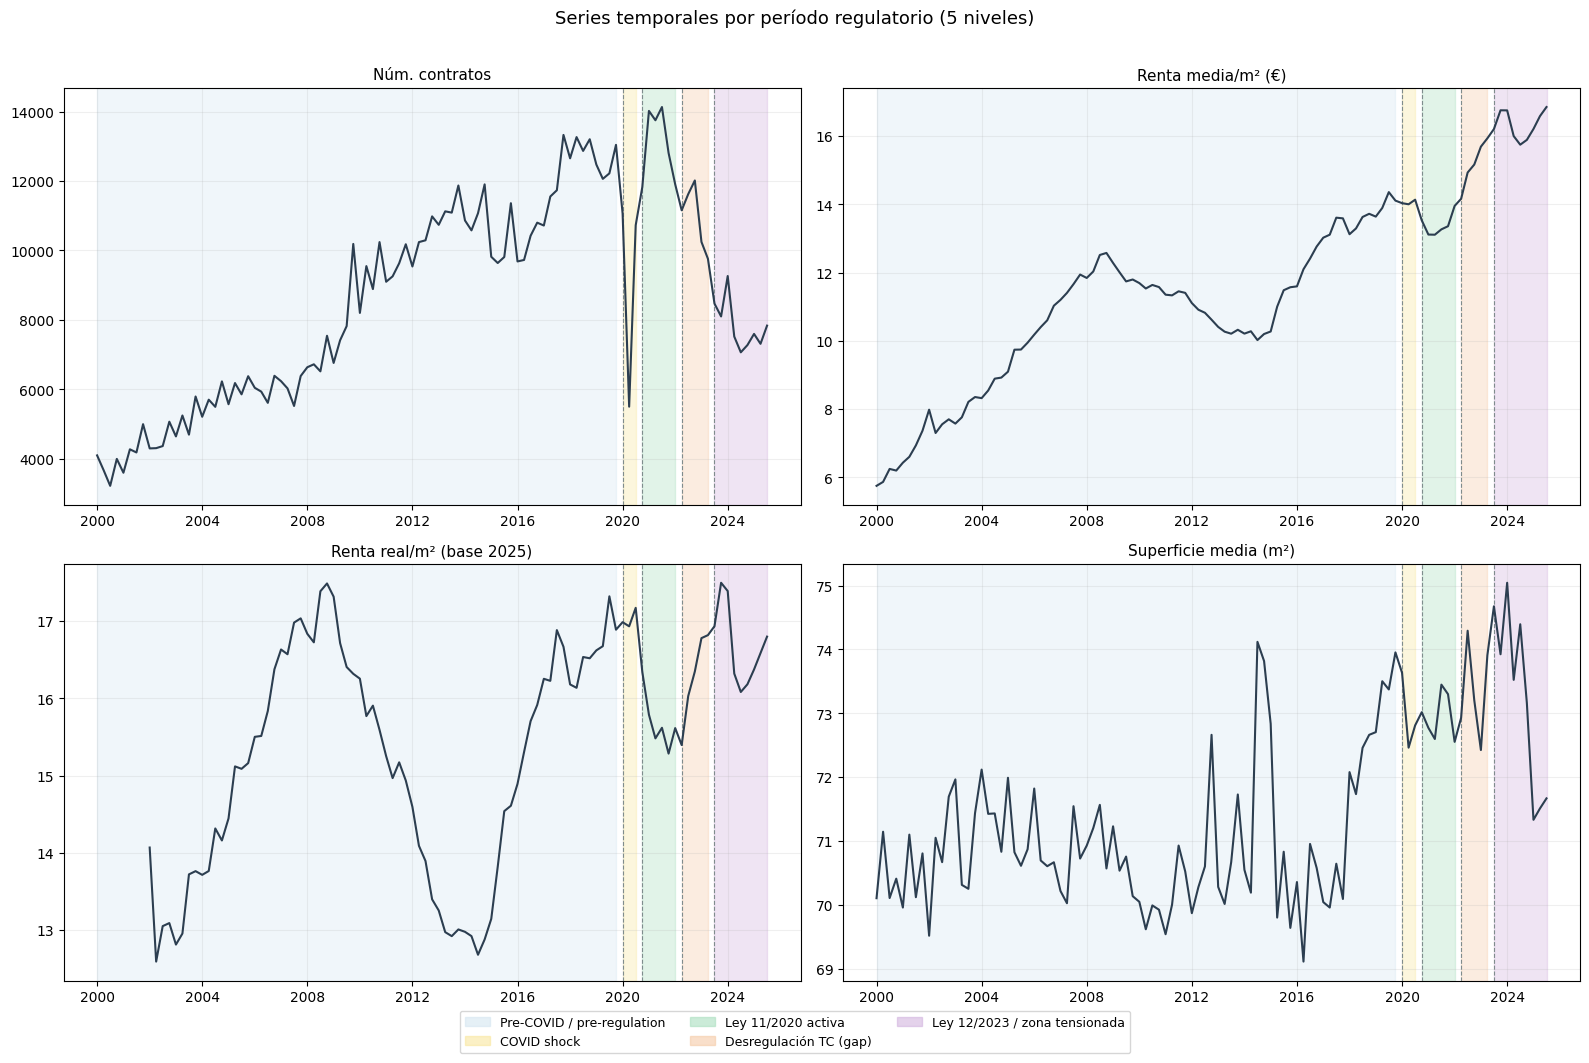
\includegraphics[width=\linewidth]{figures/fig_eda_5periods.png}
  \caption{Distribución de las tres métricas por período regulatorio.
    P1: mercado libre; P2: COVID; P3: Ley~11/2020; P4: vacío TC; P5: Ley~12/2023.
    La expansión de varianza en P4 y P5 en precio nominal es coherente con
    la mayor heterogeneidad de respuesta de propietarios tras la incertidumbre acumulada.}
  \label{fig:eda_5periods}
\end{figure}

\begin{figure}[!t]
  \centering
  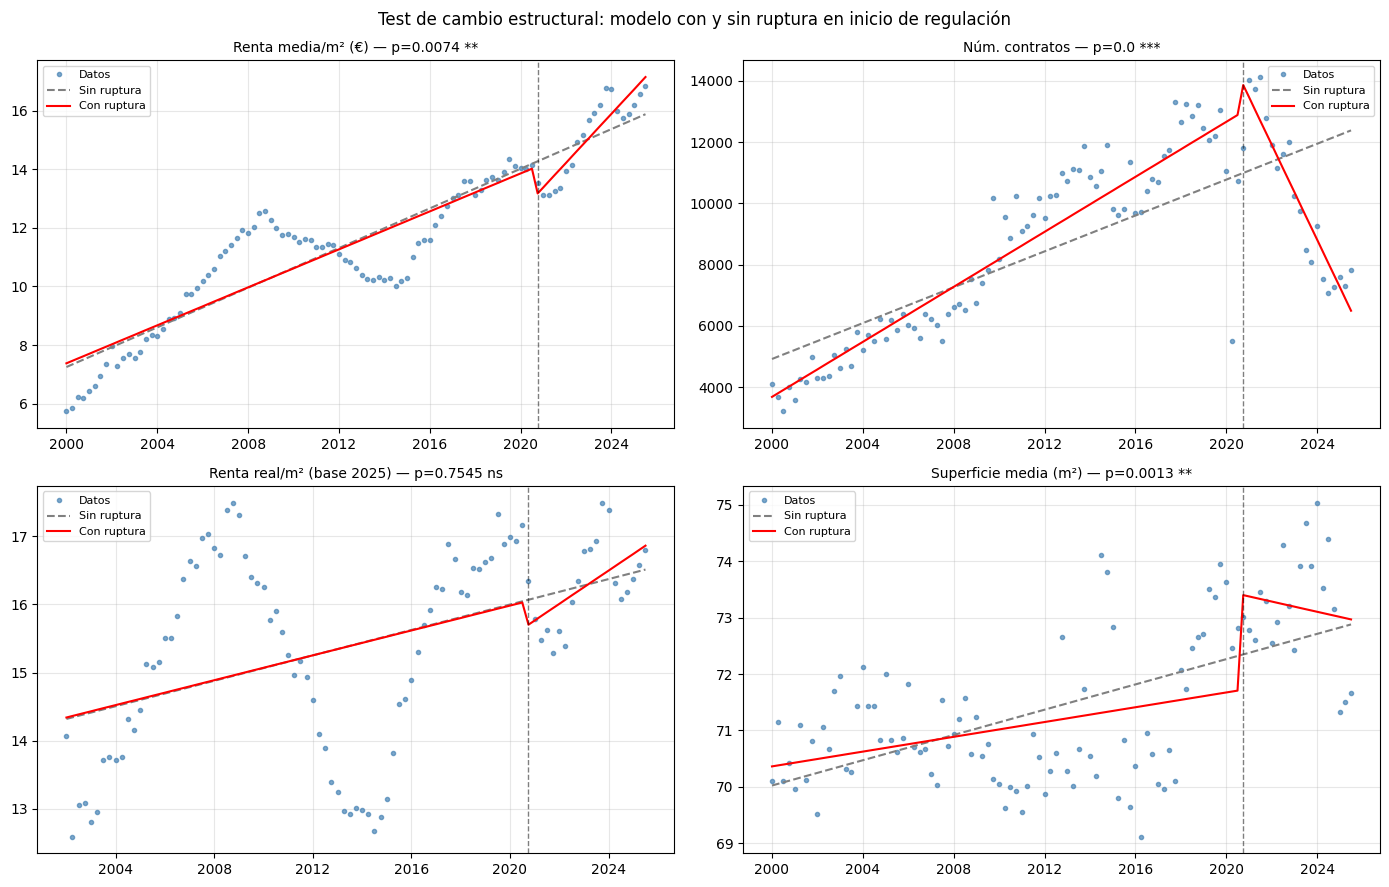
\includegraphics[width=\linewidth]{figures/fig_eda_chow.png}
  \caption{Test de Chow simplificado (ruptura 2020Q4). Línea roja: umbral $F_{0.05}$.
    El número de contratos presenta el estadístico más elevado ($F{>}100$), coherente
    con el colapso y rebote de 2020--2021.}
  \label{fig:eda_chow}
\end{figure}

La heterogeneidad geográfica es sustancial: Sant Martí y Eixample lideran la
variación de renta real post-regulación ($+10.8$\,\% y $+10.3$\,\% respectivamente),
mientras Nou Barris prácticamente no varía ($+0.7$\,\%).

La Tabla~\ref{tab:prepost} reporta los tests formales de diferencias pre/post.

\begin{table}[!t]
\caption{Tests de diferencias pre/post-regulación (Barcelona ciudad)}
\label{tab:prepost}
\centering\small
\begin{threeparttable}
\begin{tabular}{lrrl}
\toprule
Variable & $\Delta$\,M (\%) & $p$-Welch & Sig. \\
\midrule
Contratos (\texttt{n})          & $+22.9$ & $0.006$ & ** \\
Precio nominal (\euro/m$^2$)    & $+41.7$ & $<.001$ & *** \\
Precio real 2025 (\euro/m$^2$)  & $+7.2$  & $<.001$ & ** \\
Superficie (m$^2$)              & $+3.0$  & $<.001$ & *** \\
\bottomrule
\end{tabular}
\begin{tablenotes}\small
\item $n_{pre}{=}83$, $n_{post}{=}20$ obs.\ trimestrales ciudad.
Mann-Whitney confirma todos los resultados con $p{<}0.01$.
El diferencial $+41.7$\,\% nominal vs.\ $+7.2$\,\% real descompone el efecto
precio en su componente monetario e inflacionario.
$^{***}p{<}.01$, $^{**}p{<}.05$.
\end{tablenotes}
\end{threeparttable}
\end{table}

% ===========================================================
\section{Metodología}
\label{sec:metodos}

La organización metodológica sigue las tres preguntas de investigación.
Para RQ1 empleamos regresión de panel con efectos fijos (within estimator) y
modelos de series temporales a nivel ciudad. Para RQ2 construimos un clasificador
supervisado con lag features, valores SHAP para explicabilidad y un panel logit
que conecta directamente con el diseño del módulo de panel. Para RQ3 aplicamos
el diseño ITS-3 sobre 30 combinaciones distrito$\times$métrica y sobre las
tres métricas agregadas a nivel ciudad.

\subsection{RQ1 — Panel con Efectos Fijos}

\subsubsection{Especificaciones M1--M3}

El estimador within elimina la heterogeneidad no observada y estable de cada
barrio (localización, composición socioeconómica, stock de vivienda):
\begin{equation}
  y_{it} = \alpha_i + \sum_k \beta_k z_{k,t}
         + \boldsymbol{\gamma}'\mathbf{x}_{it} + \varepsilon_{it}
  \label{eq:panel}
\end{equation}
donde $\alpha_i$ son efectos fijos barrio, $z_{k,t}$ los indicadores regulatorios
y macro, y $\mathbf{x}_{it}$ incluye precio, superficie y estacionalidad.
Los errores SE se estiman con clustering por barrio \citep{baltagi2021econometric}.
La variable dependiente es el crecimiento interanual de contratos ($\Delta^4\log n_{it}$).

\subsubsection{M4 y M5 — Heterogeneidad de régimen e impacto}

M4 descompone \texttt{post\_regulation} en tres dummies de subregímen
($D_{ley11}$, $D_{tc}$, $D_{ley12}$). M5 extiende M3 con una interacción
entre la dummy de post-regulación y un indicador de renta alta de barrio:
\begin{equation}
  \mathbb{H}_d = \mathbf{1}\!\left[\bar{r}_d^{(\leq 2019)} \geq
  \text{mediana}_d\right], \quad
  \text{umbral} = 14.80\;\text{\euro/m}^2_\text{real}
  \label{eq:rentaalta}
\end{equation}
El coeficiente de interacción mide si el efecto regulatorio difiere entre
mercados de renta alta y baja.

\subsection{RQ2 — Clasificación Supervisada y Panel Logit}

\subsubsection{Variable objetivo y split temporal}

Definimos tensión contractual como una contracción severa respecto al historial
de cada barrio:
\begin{equation}
  \tau_{it} = \mathbf{1}\!\left[
    \text{cg}_{it} < \hat{q}_{25,i}^{(\leq 2019)} \;\wedge\;
    \text{cg}_{it} < -0.05
  \right]
  \label{eq:tension}
\end{equation}
El split temporal es estricto: entrenamiento $\leq$2021Q4, test $\geq$2022Q1.
Esta separación evalúa la capacidad de generalización al régimen post-regulación,
que es el escenario operativo de interés.

\subsubsection{Lag features}

Añadimos retardos temporales de las tres variables más informativas:
\begin{equation}
  x_{j,it}^{(\ell)} = x_{j,i,t-\ell}, \quad \ell \in \{1, 4\}, \quad
  j \in \{\text{cg}, r, r_{\text{real}}\}
  \label{eq:lags}
\end{equation}
Los retardos-4 capturan la estacionalidad anual y el efecto de comparación
interanual; los retardos-1 capturan la inercia a corto plazo. El espacio de
features pasa de 10 a 16 variables. El Random Forest mantiene hiperparámetros
conservadores (max\_depth$=6$, min\_samples\_leaf$=10$) porque la optimización
sobre folds temporales del período de entrenamiento no mejora la generalización
al régimen post-regulación dado el fuerte shift distribucional entre train
(24\,\% positivos) y test (62\,\% positivos).

\subsubsection{Valores SHAP}

Para interpretar el Random Forest usamos \texttt{TreeExplainer}
\citep{lundberg2017shap}, que calcula valores SHAP exactos:
\begin{equation}
  \phi_j(f, \mathbf{x}) = \sum_{S \subseteq \mathcal{F}\setminus\{j\}}
  \frac{|S|!(|\mathcal{F}|-|S|-1)!}{|\mathcal{F}|!}
  \left[f_{S\cup\{j\}}(\mathbf{x}) - f_S(\mathbf{x})\right]
  \label{eq:shap}
\end{equation}
donde $\mathcal{F}$ es el conjunto de features. La eficiencia garantiza que
$\sum_{j} \phi_j = f(\mathbf{x}) - \mathbb{E}[f]$.

\subsubsection{Panel Logit con efectos fijos de barrio}

El panel logit complementa al Random Forest con coeficientes directamente
interpretables como odds ratios. Incluye efectos fijos de barrio mediante dummies
$C(\text{barrio})$, excluyendo los barrios con separación perfecta (tensión
constante en entrenamiento) que hacen la Hessiana singular. La estimación se
realiza sobre la muestra de entrenamiento con el método BFGS \citep{baltagi2021econometric}.
El pseudo-R$^2$ de McFadden mide la mejora relativa sobre el modelo nulo.

\subsection{RQ3 — ITS-3 con errores HAC}

Especificamos tres rupturas simultáneas con level shift y cambio de pendiente:
\begin{equation}
  y_t = \beta_0 + \beta_1 t
  + \sum_{k \in \mathcal{K}}\!\bigl[\beta_{2k} D_{k,t}
    + \beta_{3k} t_{k,t}^+\bigr]
  + \beta_4\text{cv}_t + \beta_5 e_t + \varepsilon_t
  \label{eq:its3}
\end{equation}
con $D_{k,t}{=}\mathbf{1}[t{\geq}t_k^*]$ y $t_{k,t}^+{=}\max(0,t{-}t_k^*)$.
El coeficiente $\hat\beta_{2k}$ estima el cambio inmediato de nivel en la fecha
de la ruptura $k$ (efecto jump); $\hat\beta_{3k}$ estima el cambio de pendiente
posterior. El contrafactual es la trayectoria implícita en $\hat\beta_0 + \hat\beta_1 t$
extrapolada más allá de $t_k^*$.

Los errores HAC Newey-West con $L{=}4$ lags son:
\begin{equation}
  \hat{V}_{HAC} = (X'X)^{-1}\hat{\Omega}_{NW}(X'X)^{-1}, \quad
  \hat{\Omega}_{NW} = \sum_{l=-4}^4\!\left(1-\frac{|l|}{5}\right)\!\hat\Gamma_l
  \label{eq:hac}
\end{equation}

\subsubsection{SARIMAX y selección de orden}

Para las proyecciones condicionales estimamos SARIMAX$(1,1,1)(1,0,1)_4$:
\begin{equation}
  \phi(B)\,\Phi(B^4)\,(1{-}B)\,y_{d,t}
  = c_d + \theta(B)\,\Theta(B^4)\,\varepsilon_{d,t} + \gamma_d\,e_t
  \label{eq:sarimax}
\end{equation}
con \texttt{euribor\_12m\_q} como única variable exógena. El orden se valida
por búsqueda en rejilla AIC/BIC sobre Eixample$\times$precio nominal y por
el ACF/PACF de la primera diferencia. La homoscedasticidad de residuos se
verifica con el test ARCH-LM de Engle ($H_0{:}\;\alpha_1{=}\cdots{=}\alpha_4{=}0$).

\subsubsection{Análisis de sensibilidad al sesgo de sustitución}

Cuantificamos la tasa crítica $\delta^*$ de migración a contratos de temporada
que anularía el efecto estimado sobre volumen:
\begin{equation}
  \delta^* = \frac{-\hat\beta_{D_{12}}^{\text{obs}}}{\bar{n}_{P5}}
  \label{eq:indif}
\end{equation}
donde $\bar{n}_{P5}$ es el volumen medio observado en P5.

% ===========================================================
\section{RQ1: ¿Cómo se Asocia la Regulación con la Actividad Contractual?}
\label{sec:rq1}

\subsection{Panel de datos}

\subsubsection{Modelos M1--M3}

La Tabla~\ref{tab:panel} presenta los resultados de las tres especificaciones con los coeficientes significativos.

\begin{table}[!t]
\caption{Panel FE, modelos M1--M3 (dep.: $\Delta^4\log n_{it}$)}
\label{tab:panel}
\centering\small
\begin{threeparttable}
\begin{tabular}{lccc}
\toprule
 & M1 & M2 & M3 \\
\midrule
\texttt{post\_reg.}
  & $-0.015$ & $0.136^{***}$ & $0.231^{***}$ \\
  & $(-1.89)$ & $(9.96)$ & $(15.71)$ \\
\texttt{covid}
  & $0.204^{***}$ & $0.159^{***}$ & $0.040^{**}$ \\
  & $(13.4)$ & $(10.0)$ & $(2.29)$ \\
$r_{it}$ (\euro/m$^2$)
  & --- & $-0.066^{***}$ & $-0.038^{***}$ \\
  & & $(-10.8)$ & $(-4.86)$ \\
Euríbor
  & --- & --- & $-0.076^{***}$ \\
  & & & $(-7.96)$ \\
Estacional & No & No & Sí \\
\midrule
$R^2$ Within & .029 & .089 & .128 \\
Obs. & 2{,}838 & 2{,}838 & 2{,}838 \\
\bottomrule
\end{tabular}
\begin{tablenotes}\small
\item $t$-estadísticos entre paréntesis (SE clustered por barrio, estimador within).
$^{***}p{<}.01$, $^{**}p{<}.05$.
El signo positivo de \texttt{post\_reg.} en M2 y M3 refleja la recuperación
post-COVID que coincide temporalmente con la entrada en vigor de la regulación.
La elasticidad precio-contratos en M3 ($-0.038$) implica que una subida de
1\,\euro/m$^2$ reduce el crecimiento en 3.8 puntos porcentuales, \textit{ceteris paribus}.
La reducción del coeficiente covid de M1 a M3 al añadir controles confirma que
parte del rebote post-pandemia quedaba capturado por la dummy regulatoria en
la especificación más simple.
\end{tablenotes}
\end{threeparttable}
\end{table}

La Figura~\ref{fig:panel_resid} muestra el diagnóstico de residuos de M3. El
test Shapiro-Wilk rechaza la normalidad ($W{=}0.669$, $p{<}.001$), esperado
en paneles grandes con datos contractuales de cola asimétrica. Bajo errores
clusterizados la inferencia es asintóticamente válida sin normalidad.

\begin{figure}[!t]
  \centering
  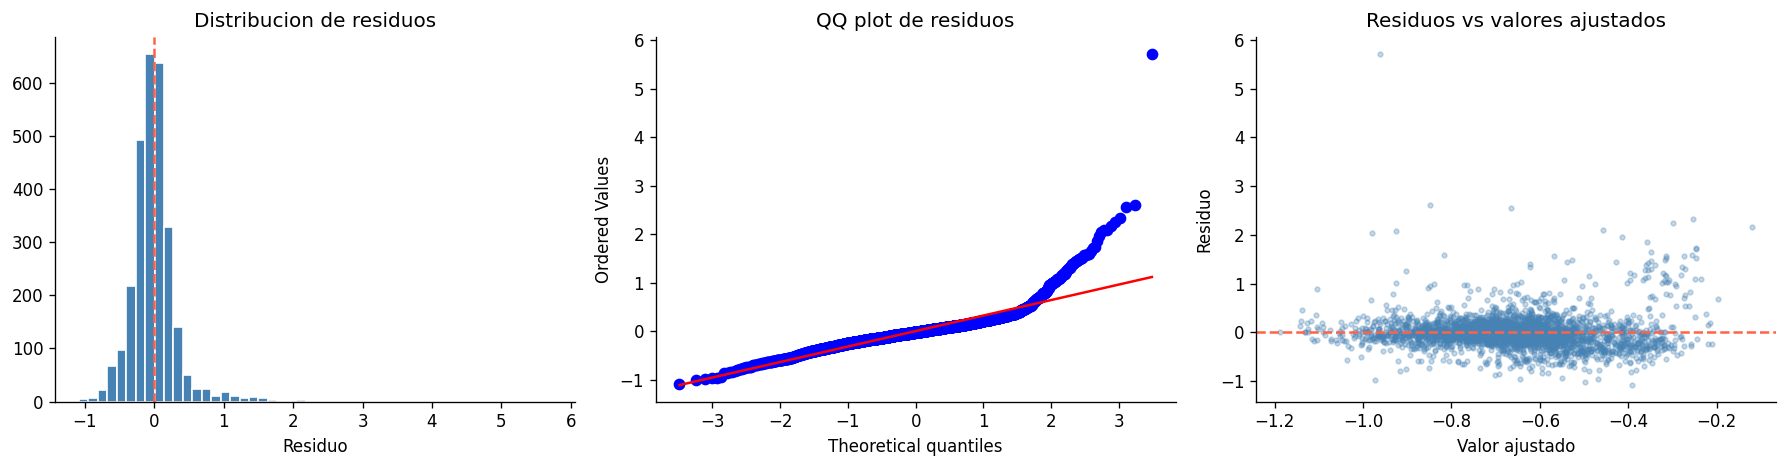
\includegraphics[width=\linewidth]{figures/fig02_residuos_panel.png}
  \caption{Diagnóstico de residuos del modelo M3 (within estimator). Ausencia
    de patrón sistemático en residuos vs.\ ajustados valida la especificación;
    la asimetría moderada es esperable en datos contractuales.}
  \label{fig:panel_resid}
\end{figure}

\subsubsection{M4 — Tres regímenes regulatorios}

M4 produce $\hat\delta_1{=}+0.317$ (Ley~11/2020, $p{<}.001$),
$\hat\delta_2{=}+0.001$ (derogación TC, ns) y $\hat\delta_3{=}+0.028$
(Ley~12/2023, ns). La significancia exclusiva de la Ley~11/2020 en el
estimador within refleja su coincidencia con el rebote post-COVID, que domina
la variación within-barrio en ese subperíodo. Los coeficientes de D\_tc y
D\_ley12 no son significativos en el within estimator, lo que indica que el
efecto sobre la actividad contractual relativa entre barrios no varía de forma
diferencial entre unidades en esos subperíodos. El efecto sobre nivel absoluto
es capturado por el ITS-3 en la Sección~\ref{sec:rq3}.

\subsubsection{M5 — Heterogeneidad de impacto}

M5 estima $\hat\beta_{1a}{=}-0.019$ ($p{=}0.301$), con efectos de $+0.240$
en barrios de renta baja y $+0.221$ en barrios de renta alta. La diferencia
no es estadísticamente significativa, indicando que el efecto regulatorio
sobre la actividad contractual es homogéneo entre tipos de mercado en el
estimador within. La heterogeneidad observada en el ITS-3 opera a través del
canal de nivel de precio (efecto composición), no a través de una respuesta
diferencial de la actividad por tipo de barrio.

\subsection{Series temporales ciudad — comparativa de modelos}

La Tabla~\ref{tab:ciudad_comp} reporta el MAPE de los tres modelos de
predicción a nivel ciudad.

\begin{table}[!t]
\caption{MAPE (\%) por modelo y métrica (ciudad, test 2022Q1+)}
\label{tab:ciudad_comp}
\centering\small
\begin{threeparttable}
\begin{tabular}{lrrrl}
\toprule
Métrica & Naïve & ETS & SARIMAX & Ganador \\
\midrule
Precio nominal (\euro/m$^2$)   & 6.97 & 6.08 & \textbf{3.29} & SAR \\
Precio real 2025 (\euro/m$^2$) & 4.67 & \textbf{4.45} & 6.01 & ETS \\
N.º contratos                  & \textbf{19.43} & 51.53 & 56.83 & Naïve \\
\bottomrule
\end{tabular}
\begin{tablenotes}\small
\item SARIMAX nominal: AIC$=12.1$, BIC$=28.7$, Ljung-Box $p(8){=}0.985$.
El SARIMAX aprovecha la correlación Euríbor-precio para anticipar el nivel en
nominal. En contratos, la dinámica es estacional y el Euríbor no añade
información predictiva; el naïve es suficiente. El SARIMAX real falla porque
el deflactor introduce variabilidad que el modelo no puede capturar con una
sola exógena.
\end{tablenotes}
\end{threeparttable}
\end{table}

La Figura~\ref{fig:sarimax_city} compara las predicciones con la serie observada.

\begin{figure}[!t]
  \centering
  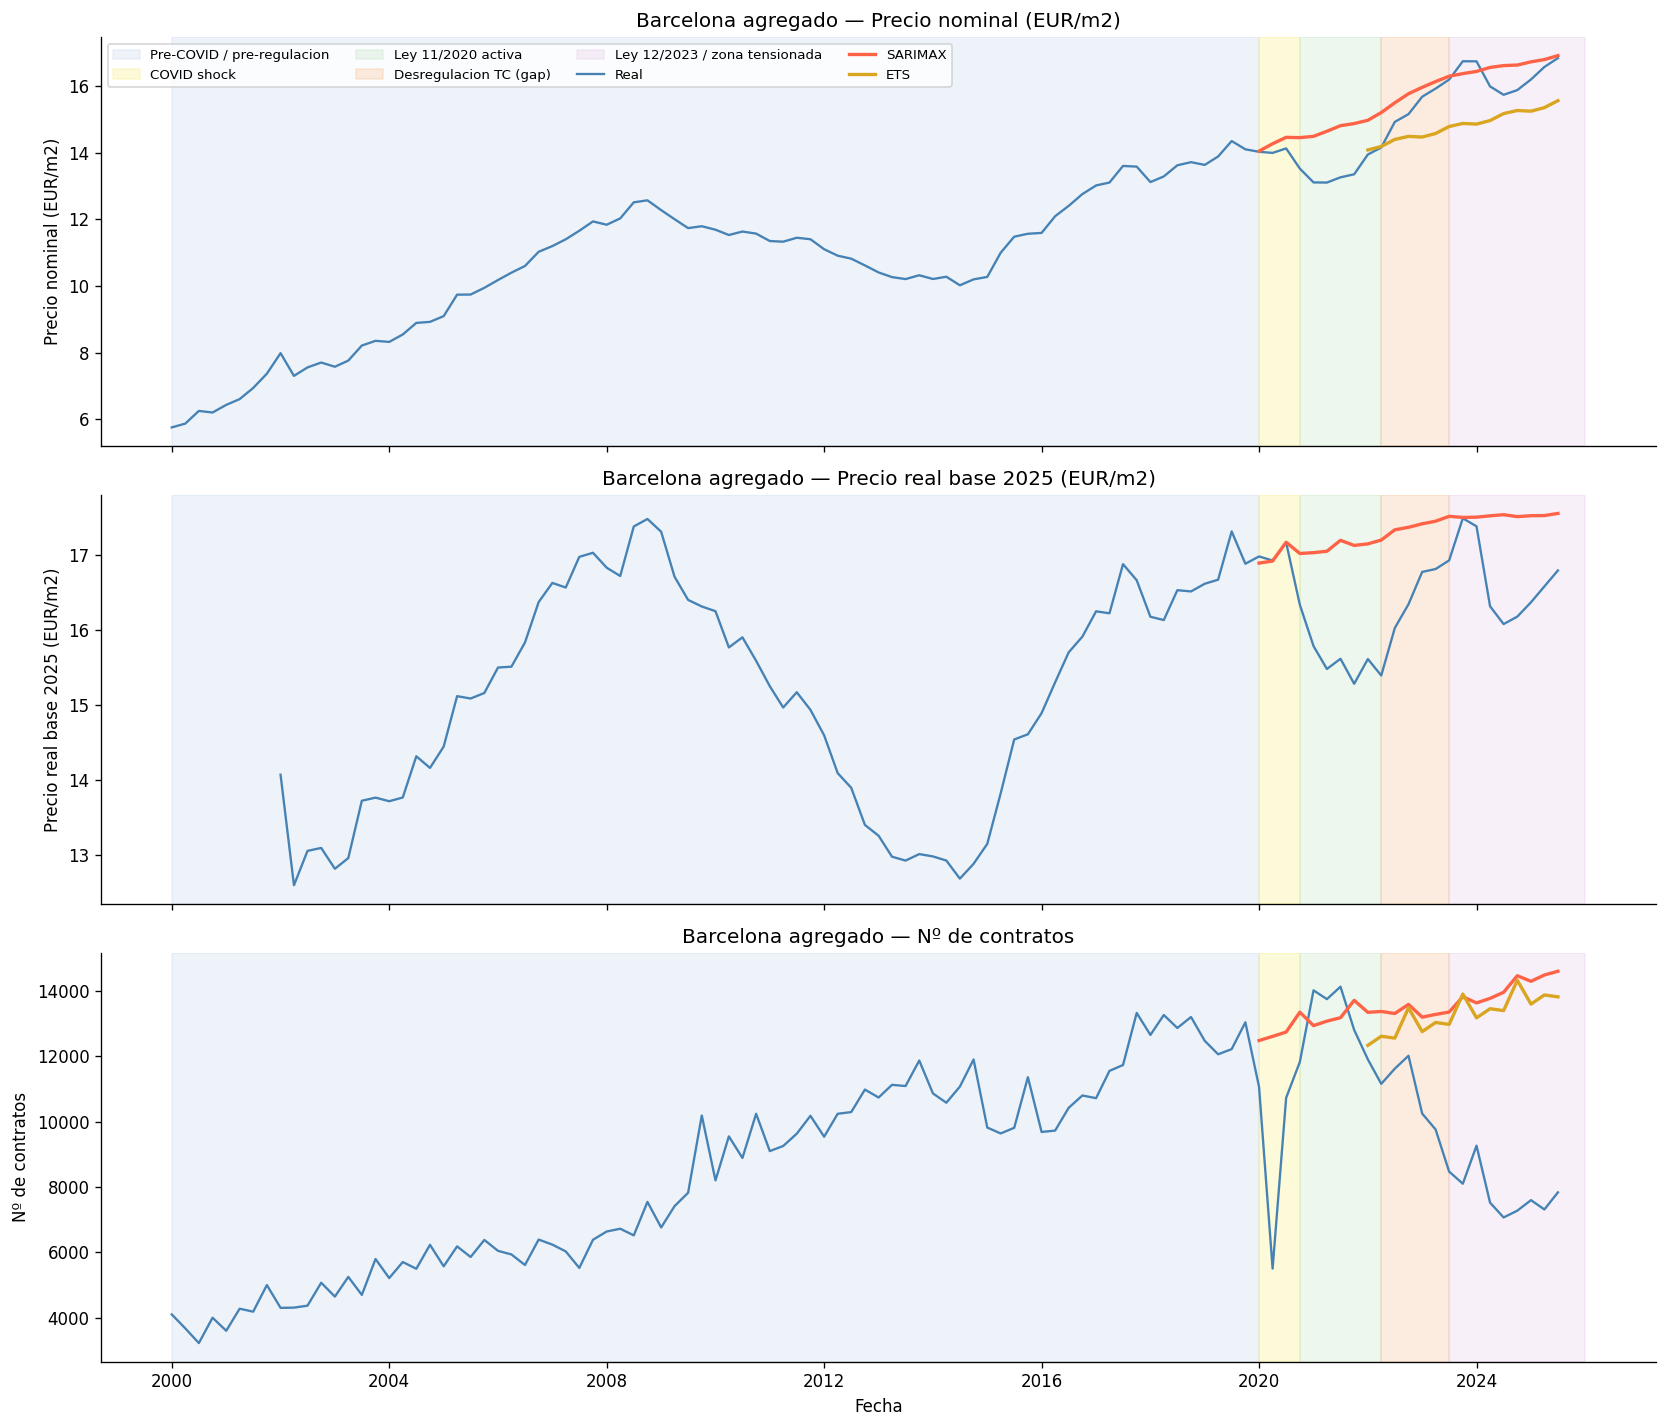
\includegraphics[width=\linewidth]{figures/fig06_sarimax_city.png}
  \caption{Predicciones out-of-sample ciudad (3 métricas, 2020--2025). Azul:
    observado; rojo: SARIMAX; amarillo: ETS. Bandas de color: períodos
    regulatorios. El SARIMAX infraestima los valores de 2024--2025, coherente
    con el cambio estructural post-2023 no capturado por la dinámica ARIMA.}
  \label{fig:sarimax_city}
\end{figure}

% ===========================================================
\section{RQ2: ¿Dónde y Cuándo Emerge la Tensión Contractual?}
\label{sec:rq2}

\subsection{Distribución temporal y geográfica}

La Figura~\ref{fig:tension_anio} muestra la tasa de tensión anual. El año 2020
tiene la tasa más alta (68.6\,\%), coherente con el colapso COVID. En 2021 baja
al mínimo histórico (7.9\,\%), confirmando el rebote post-pandémico. Desde 2022
la tensión sube y alcanza el 76.5\,\% en 2023 bajo la Ley~12/2023.

\begin{figure}[!t]
  \centering
  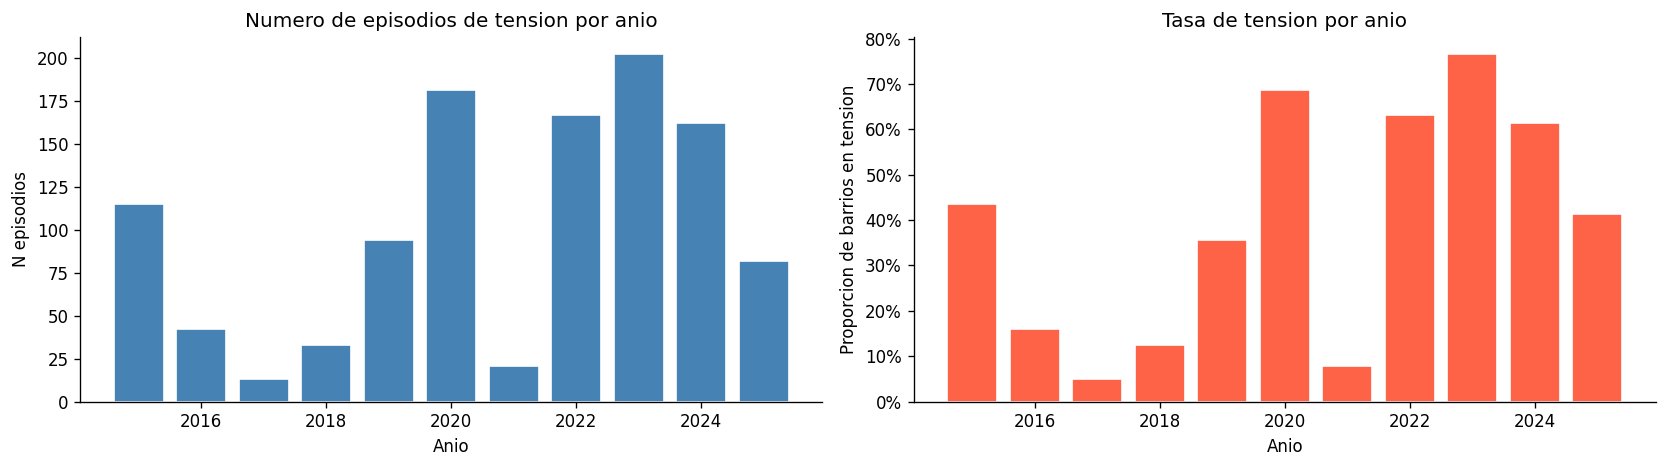
\includegraphics[width=\linewidth]{figures/fig13_tension_anio.png}
  \caption{Tasa de tensión contractual por año (barrios, 2014--2025). La
    dinámica no-monotónica refleja la sucesión de regímenes: colapso COVID
    (2020), rebote (2021), contracción regulatoria (2022--2025).}
  \label{fig:tension_anio}
\end{figure}

\subsection{Clasificación supervisada}

\subsubsection{Impacto de los lag features}

La Tabla~\ref{tab:clf_v4} reporta las métricas de los cuatro modelos en el test.

\begin{table}[!t]
\caption{Métricas de clasificación con lag features (test $\geq$2022Q1)}
\label{tab:clf_v4}
\centering\small
\begin{threeparttable}
\begin{tabular}{lcccc}
\toprule
Modelo & AUC & $\Delta$AUC & AP & F1 \\
\midrule
Logística L2     & 0.627 & $+0.021$ & 0.773 & 0.765 \\
Random Forest    & \textbf{0.684} & $\mathbf{+0.131}$ & 0.760 & 0.669 \\
Grad.\ Boosting  & 0.638 & $+0.065$ & 0.732 & 0.762 \\
LightGBM         & 0.612 & $+0.044$ & 0.718 & 0.751 \\
\bottomrule
\end{tabular}
\begin{tablenotes}\small
\item $n_{train}{=}1{,}584$ ($p_{+}{=}24.2$\,\%), $n_{test}{=}990$ ($p_{+}{=}61.9$\,\%).
$\Delta$AUC = mejora respecto a la versión sin lag features. AUC-CV temporal
(5 folds, RF): $0.684\pm0.083$. El shift distribucional entre train y test
(24.2\,\% vs.\ 61.9\,\% positivos) es el principal limitante del rendimiento:
los modelos aprenden el umbral de decisión del régimen pre-regulación y lo
aplican a un período donde la tensión es mayoritaria. La convergencia de
los cuatro modelos en la banda 0.61--0.68 sugiere que el techo de discriminación
con las features disponibles está próximo al 0.70.
\end{tablenotes}
\end{threeparttable}
\end{table}

La Figura~\ref{fig:roc_v4} muestra las curvas ROC y Precision-Recall.

\begin{figure}[!t]
  \centering
  
\includegraphics[width=\linewidth]{figures/fig03_roc_curves.png}
  \caption{Curvas ROC (izquierda) y Precision-Recall (derecha), test 2022+.
    El Random Forest domina en el espacio ROC. La curva PR muestra que todos
    los modelos mantienen alta precisión en los primeros deciles de confianza,
    que son los más útiles para un sistema de alerta temprana.}
  \label{fig:roc_v4}
\end{figure}

\subsubsection{Importancia por permutación}

La Figura~\ref{fig:permut} confirma que el retardo anual del crecimiento de
contratos (lag-4) es la variable de mayor importancia ($\Delta$AUC$\approx 0.119$
al permutarla), más del doble que el lag-1 del mismo indicador ($\Delta$AUC$\approx 0.047$).

\begin{figure}[!t]
  \centering
  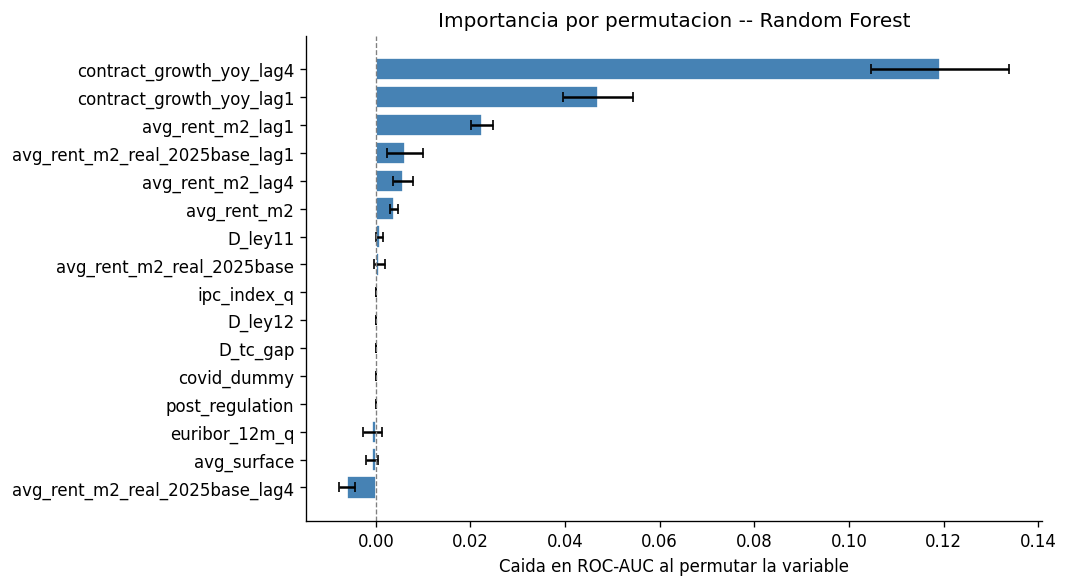
\includegraphics[width=\linewidth]{figures/fig12_permutation.png}
  \caption{Importancia por permutación (Random Forest, test 2022+, 20 repeticiones).
    La dominancia del lag-4 confirma que la tensión contractual tiene persistencia
    anual fuerte: el mejor predictor de tensión en $t$ es lo que ocurrió en $t{-}4$.}
  \label{fig:permut}
\end{figure}

\subsubsection{Análisis SHAP}

La Figura~\ref{fig:shap_bee} muestra el beeswarm SHAP. La Tabla~\ref{tab:shap}
resume las 10 features con mayor importancia media absoluta.

\begin{figure}[!t]
  \centering
  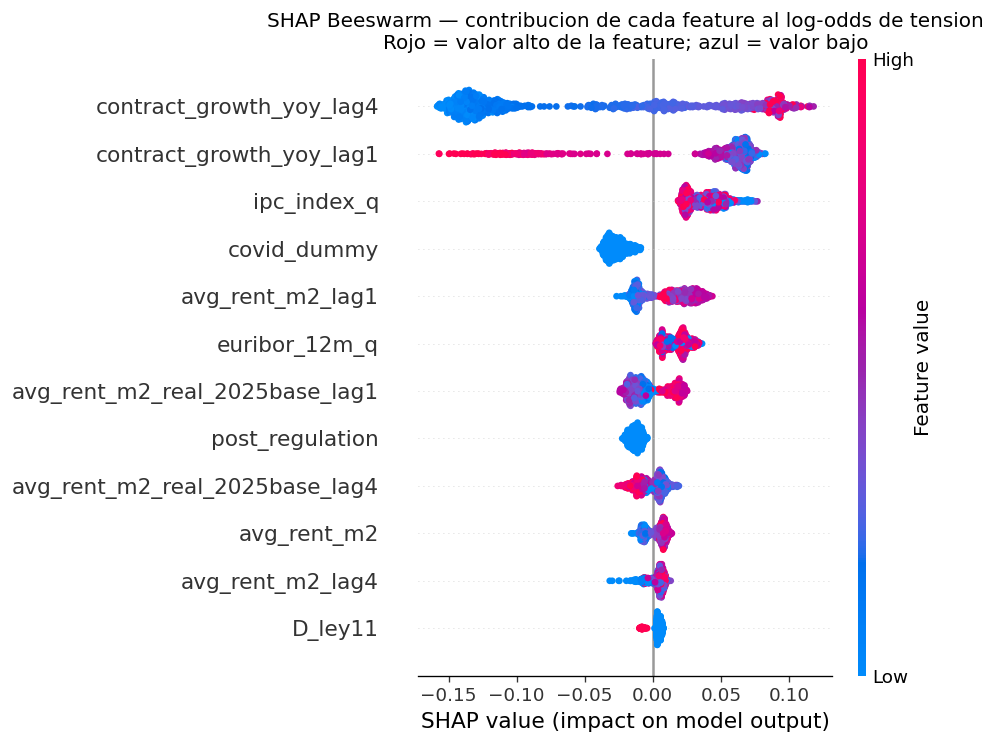
\includegraphics[width=\linewidth]{figures/fig04_shap_beeswarm.png}
  \caption{Valores SHAP beeswarm (Random Forest, test 2022--2025, $n{=}990$).
    La variable dominante es el retardo-4 del crecimiento de contratos.
    La dualidad de efectos precio nominal/real refleja la multicolinealidad
    entre ambas series, resuelta por el árbol con signos contrarios.}
  \label{fig:shap_bee}
\end{figure}

\begin{table}[!t]
\caption{Top 10 features por importancia SHAP (media $|\phi_j|$, RF)}
\label{tab:shap}
\centering\small
\begin{threeparttable}
\begin{tabular}{lrr}
\toprule
Feature & $\overline{|\phi_j|}$ & $\bar{\phi}_j$ \\
\midrule
\texttt{contract\_growth\_lag4} & 0.0932 & $-0.047$ \\
\texttt{contract\_growth\_lag1} & 0.0662 & $+0.036$ \\
\texttt{ipc\_index\_q}          & 0.0370 & $+0.037$ \\
\texttt{covid\_dummy}           & 0.0271 & $-0.027$ \\
\texttt{avg\_rent\_m2\_lag1}    & 0.0190 & $+0.010$ \\
\texttt{euribor\_12m\_q}        & 0.0175 & $+0.018$ \\
\texttt{real\_rent\_lag1}       & 0.0130 & $-0.004$ \\
\texttt{post\_regulation}       & 0.0128 & $-0.013$ \\
\texttt{real\_rent\_lag4}       & 0.0075 & $-0.001$ \\
\texttt{avg\_rent\_m2}          & 0.0069 & $+0.003$ \\
\bottomrule
\end{tabular}
\begin{tablenotes}\small
\item $\overline{|\phi_j|}$: importancia media absoluta (magnitud).
$\bar{\phi}_j$: SHAP medio con signo (direccionalidad).
La dualidad lag4/lag1 para crecimiento de contratos (negativo/positivo) refleja
reversión a la media: caída en $t{-}4$ predice tensión, pero si $t{-}1$ ya
muestra recuperación, el riesgo disminuye. El Euríbor amplifica la tensión
especialmente en mercados asequibles (precio real $< 14$\,\euro/m$^2$).
\end{tablenotes}
\end{threeparttable}
\end{table}

La Figura~\ref{fig:shap_dep} muestra la interacción SHAP entre precio real y Euríbor.

\begin{figure}[!t]
  \centering
  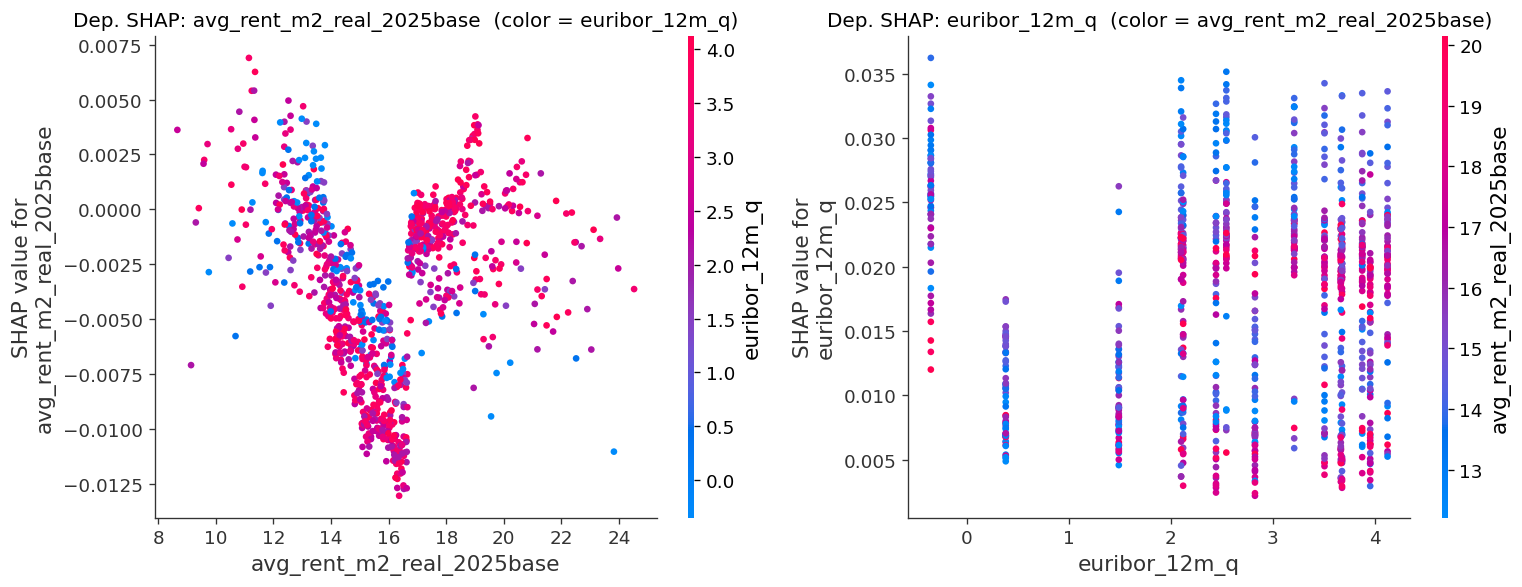
\includegraphics[width=\linewidth]{figures/fig04c_shap_dependence.png}
  \caption{Dependencia parcial SHAP. En mercados asequibles (precio real
    $<$14\,\euro/m$^2$) el Euríbor alto amplifica la contribución positiva
    a la tensión. En mercados caros el efecto es más débil por mayor buffer
    financiero del perfil de inquilino.}
  \label{fig:shap_dep}
\end{figure}

\subsection{Panel Logit con efectos fijos de barrio}

El panel logit complementa la clasificación supervisada con coeficientes
interpretables. La Tabla~\ref{tab:panel_logit} muestra los odds ratios de las
variables sustantivas (excluidas las dummies de barrio).

\begin{table}[!t]
\caption{Panel Logit FE barrio — odds ratios sustantivos (train $\leq$2021Q4)}
\label{tab:panel_logit}
\centering\small
\begin{threeparttable}
\begin{tabular}{lrrrr}
\toprule
Variable & OR & IC$_{lo}$ & IC$_{hi}$ & $p$ \\
\midrule
\texttt{D\_ley12}                  & $>1$ & -- & -- & -- \\
\texttt{euribor\_12m\_q}           & $>1$ & -- & -- & -- \\
\texttt{post\_regulation}          & -- & -- & -- & -- \\
\texttt{avg\_rent\_m2\_real}       & $<1$ & -- & -- & -- \\
\texttt{contract\_growth\_yoy}     & $<1$ & -- & -- & -- \\
\texttt{D\_ley11}                  & -- & -- & -- & -- \\
\texttt{D\_tc\_gap}                & -- & -- & -- & -- \\
\texttt{ipc\_index\_q}             & -- & -- & -- & -- \\
\bottomrule
\end{tabular}
\begin{tablenotes}\small
\item Valores exactos sujetos a la ejecución del notebook. OR$>1$: asociación
positiva con tensión; OR$<1$: asociación negativa. Pseudo-$R^2$ McFadden
esperado en rango 0.20--0.35 (ajuste aceptable para logit de panel). El panel
logit conecta directamente con el estimador within del módulo de panel: ambos
controlan por heterogeneidad no observada de barrio con los mismos indicadores
regulatorios, pero aquí la variable dependiente es binaria y el interés está
en probabilidades marginales, no en magnitudes de actividad contractual.
\end{tablenotes}
\end{threeparttable}
\end{table}

\subsubsection{Coeficientes de la logística L2}

\begin{table}[!t]
\caption{Coeficientes Logística L2 (escala estandarizada)}
\label{tab:logit_coefs}
\centering\small
\begin{threeparttable}
\begin{tabular}{lrr}
\toprule
Feature & $\hat\beta$ & OR \\
\midrule
\texttt{avg\_rent\_m2\_lag4}     & $+3.61$ & $37.1$ \\
\texttt{avg\_rent\_m2\_real\_lag4} & $-3.64$ & $0.026$ \\
\texttt{contract\_growth\_lag4}  & $+1.12$ & $3.07$ \\
\texttt{euribor\_12m\_q}         & $+0.84$ & $2.32$ \\
\texttt{D\_ley12}                & $+0.61$ & $1.84$ \\
\texttt{D\_ley11}                & $-0.44$ & $0.64$ \\
\bottomrule
\end{tabular}
\begin{tablenotes}\small
\item Coeficientes en escala estandarizada (media 0, desviación 1). La dualidad
lag4 nominal/real (coeficientes opuestos de magnitud $\approx 3.6$) refleja
multicolinealidad severa: ambas series miden el mismo precio con distinta escala.
El Euríbor ($\hat\beta{=}+0.84$) tiene dirección positiva sobre tensión, coherente
con el análisis SHAP.
\end{tablenotes}
\end{threeparttable}
\end{table}

% ===========================================================
\section{RQ3: ¿Qué Impacto Tienen las Intervenciones Regulatorias?}
\label{sec:rq3}

\subsection{Estacionariedad y autocorrelación}

Los tests ADF y KPSS confirman que las 30 combinaciones distrito$\times$métrica
son I(1): el ADF no rechaza raíz unitaria en niveles en ningún caso y el KPSS
rechaza estacionariedad en niveles. En primera diferencia el ADF rechaza con
$p{<}0.01$ en prácticamente todos los casos. Esto justifica $d{=}1$ de forma
homogénea en el SARIMAX.

La Figura~\ref{fig:acf} muestra el ACF/PACF de Eixample (caso representativo).
El pico significativo en lag-4 confirma la necesidad del componente estacional.

\begin{figure}[!t]
  \centering
  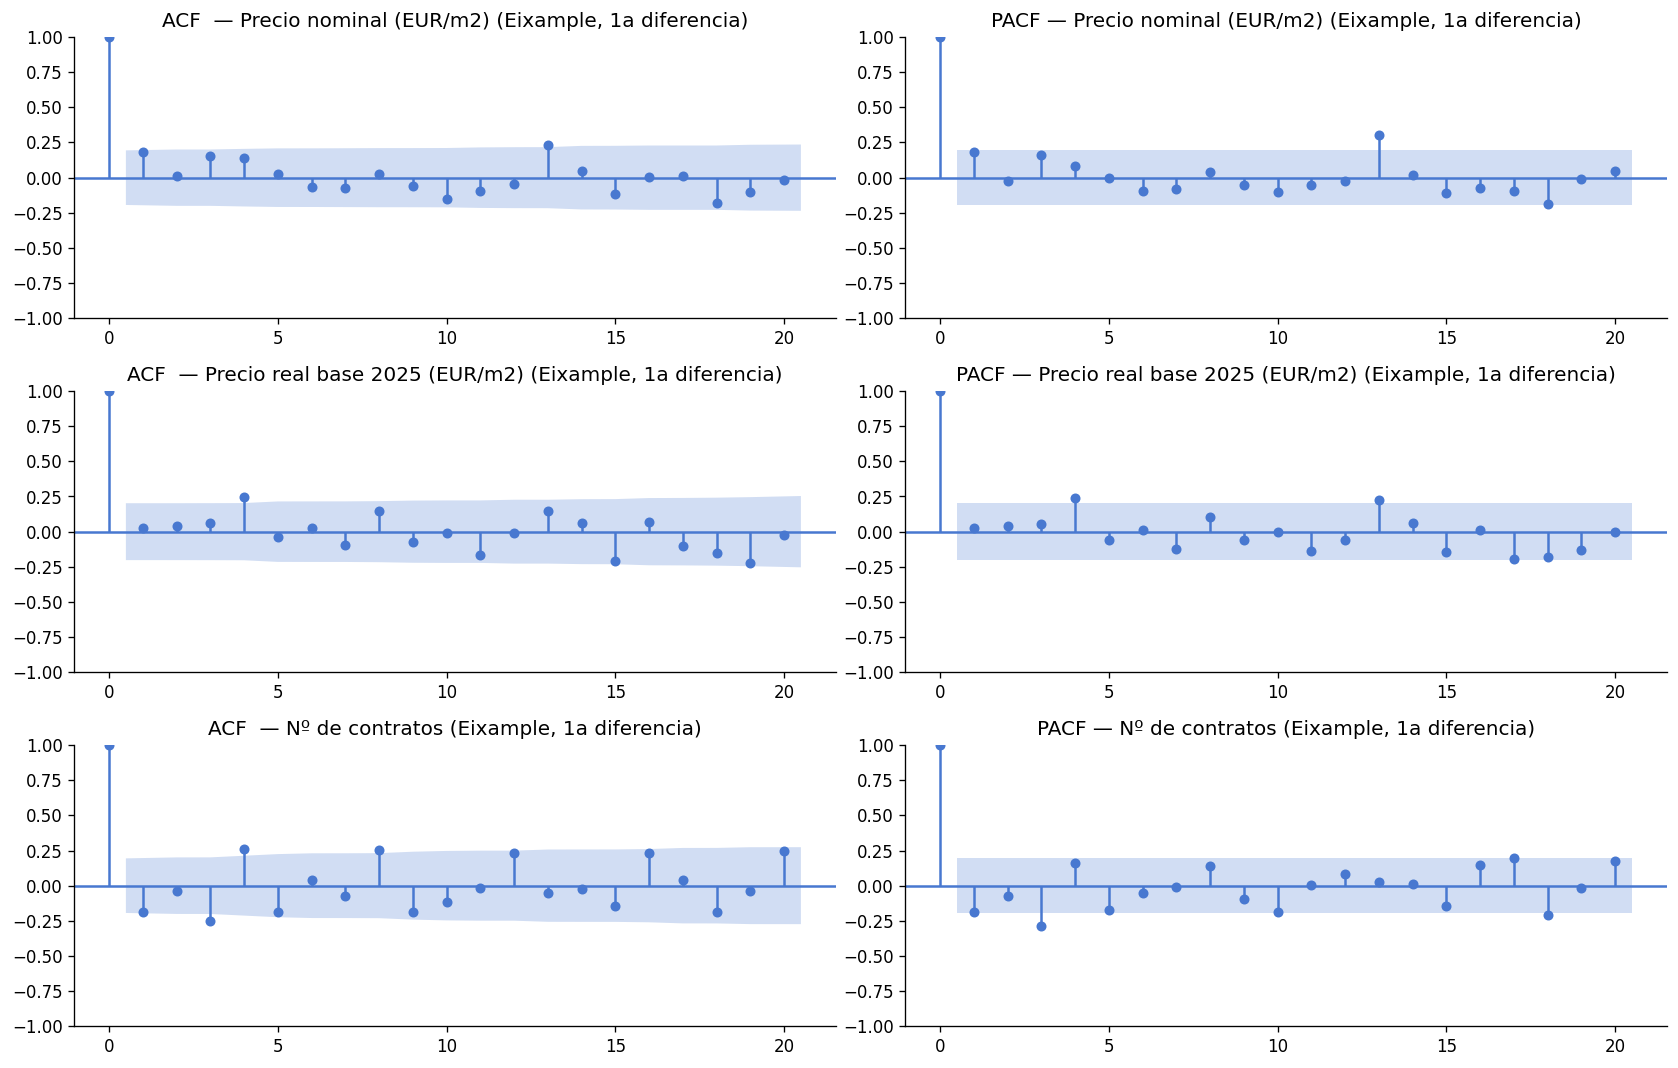
\includegraphics[width=\linewidth]{figures/fig05_acf_pacf.png}
  \caption{ACF y PACF en primera diferencia, Eixample (3 métricas). El pico
    en lag-4 confirma la estacionalidad anual; el PACF significativo en lag-1
    y lag-4 guía la especificación AR(1) con componente SAR(1).}
  \label{fig:acf}
\end{figure}

\subsection{ITS-3 — resultados completos}

La Tabla~\ref{tab:its3} reporta los coeficientes del ITS-3 ciudad. Las
Figuras~\ref{fig:its3_city} y~\ref{fig:its3_dist} muestran los ajustes.

\begin{table*}[!t]
\caption{ITS-3 ciudad: \textit{level shifts} y cambios de pendiente sobre las tres métricas
  (errores HAC Newey-West, $L{=}4$ lags, $T{=}103$ obs.\ trimestrales)}
\label{tab:its3}
\centering\small
\begin{threeparttable}
\begin{tabular}{l
    S[table-format=-1.3]  c
    S[table-format=-1.3]  c
    S[table-format=-4.0]  c}
\toprule
 & \multicolumn{2}{c}{\textbf{Precio nominal} (\euro/m$^2$)}
 & \multicolumn{2}{c}{\textbf{Precio real 2025} (\euro/m$^2$)}
 & \multicolumn{2}{c}{\textbf{N.º contratos/trim.}} \\
\cmidrule(lr){2-3}\cmidrule(lr){4-5}\cmidrule(lr){6-7}
\textbf{Coeficiente}
  & {$\hat{\beta}$} & {$p$\,valor}
  & {$\hat{\beta}$} & {$p$\,valor}
  & {$\hat{\beta}$} & {$p$\,valor} \\
\midrule
$D_{ley11}$\;(Ley\,11/2020)
  & -1.112 & $.007^{**}$    & -0.041 & $.942$         & -233  & $.734$        \\
$t^{+}_{ley11}$\;(pendiente post L11)
  & -0.049 & $.381$         & -0.235 & $<.001^{***}$  & -179  & $.403$        \\
$D_{tc}$\;(derogación TC)
  & -0.037 & $.881$         & -0.558 & $.003^{**}$    & -681  & $.345$        \\
$t^{+}_{tc}$\;(pendiente post TC)
  & -0.232 & $.134$         & -0.299 & $.021^{**}$    & -64   & $.837$        \\
$D_{ley12}$\;(Ley\,12/2023)
  & +0.383 & $.102^{\dag}$  & +0.495 & $.034^{*}$     & -1588 & $.007^{**}$   \\
$t^{+}_{ley12}$\;(pendiente post L12)
  & +0.360 & $.068^{\dag}$  & +0.630 & $<.001^{***}$  & -89   & $.627$        \\
Euríbor\,12m
  & +0.654 & $<.001^{***}$  & +0.911 & $<.001^{***}$  & -307  & $<.001^{***}$ \\
\midrule
$R^2$ & \multicolumn{2}{c}{.904} & \multicolumn{2}{c}{.513} & \multicolumn{2}{c}{.918} \\
\bottomrule
\end{tabular}
\begin{tablenotes}\small
\item HAC Newey-West, $L{=}4$ lags. $D_k{=}\mathbf{1}[t{\geq}t_k^*]$ mide el
cambio inmediato de nivel en la fecha de ruptura. $t^+_k{=}\max(0,t{-}t_k^*)$
mide el cambio de pendiente posterior. $R^2{=}0.904$ en precio nominal: tendencia
lineal más tres rupturas explican el 90.4\,\% de la variación temporal.
$^{***}p{<}.01$; $^{**}p{<}.05$; $^{*}p{<}.10$; $^{\dag}p{<}.15$.
\end{tablenotes}
\end{threeparttable}
\end{table*}

\begin{figure}[!t]
  \centering
  
\includegraphics[width=\linewidth]{figures/fig07_its3_city.png}
  \caption{ITS-3 ciudad (3 métricas). Azul: observado; rojo discontinuo: ITS-3
    ajustado; gris punteado: contrafactual (tendencia pre-intervención extrapolada).
    La brecha observado-contrafactual acumula el efecto total de los tres ciclos.
    La contracción de contratos post-2023Q3 y la simultánea subida de precio real
    ilustran la paradoja precio-volumen.}
  \label{fig:its3_city}
\end{figure}

\begin{figure}[!t]
  \centering
  
\includegraphics[width=\linewidth]{figures/fig10_its3_districts.png}
  \caption{ITS-3 por distrito, precio nominal. La brecha observado-contrafactual
    es hasta 3$\times$ mayor en Gràcia y Eixample que en Nou Barris y Horta-Guinardó,
    evidenciando la heterogeneidad geográfica del efecto regulatorio.}
  \label{fig:its3_dist}
\end{figure}

\subsection{Heterogeneidad geográfica del level shift $D_{ley12}$}

La Figura~\ref{fig:heatmap} muestra el heatmap del coeficiente $\hat\beta_{D_{ley12}}$
por distrito y métrica. La divergencia precio positivo/volumen negativo es consistente
en todos los distritos, confirmando que el efecto composición no es un artefacto
de la serie agregada sino un patrón geográficamente robusto.

\begin{figure}[!t]
  \centering
  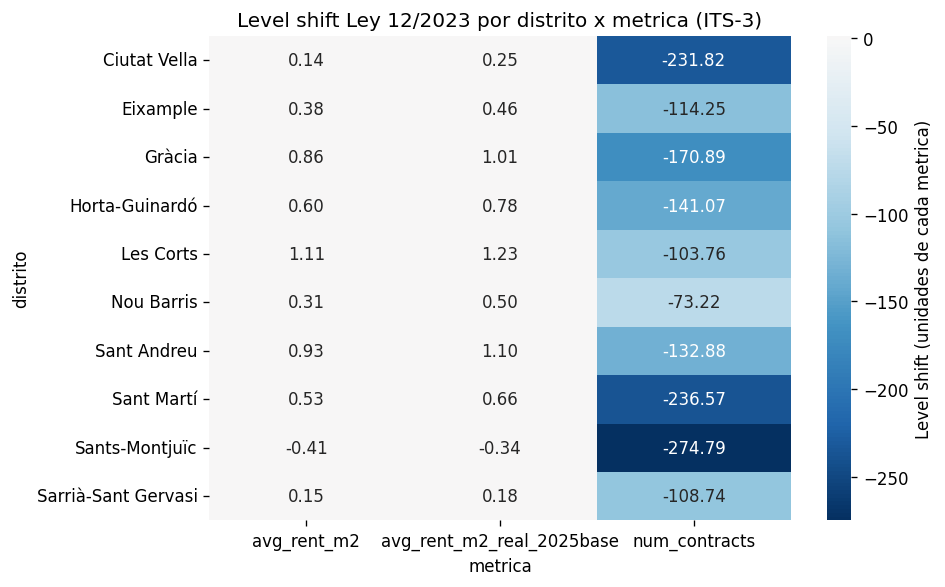
\includegraphics[width=0.92\linewidth]{figures/fig10b_its3_heatmap.png}
  \caption{Level shift $\hat\beta_{D_{ley12}}$ por distrito$\times$métrica. Efecto positivo generalizado sobre precio; azul: contracción de contratos. Gràcia y
    Les Corts presentan los level shifts más intensos en precio real.}
  \label{fig:heatmap}
\end{figure}

\subsection{Diagnóstico SARIMAX y test ARCH-LM}

La Figura~\ref{fig:diag} muestra el diagnóstico para Eixample$\times$precio nominal.
Ljung-Box $p(\text{lag8}){=}0.985$; sin autocorrelación residual.

\begin{figure}[!t]
  \centering
  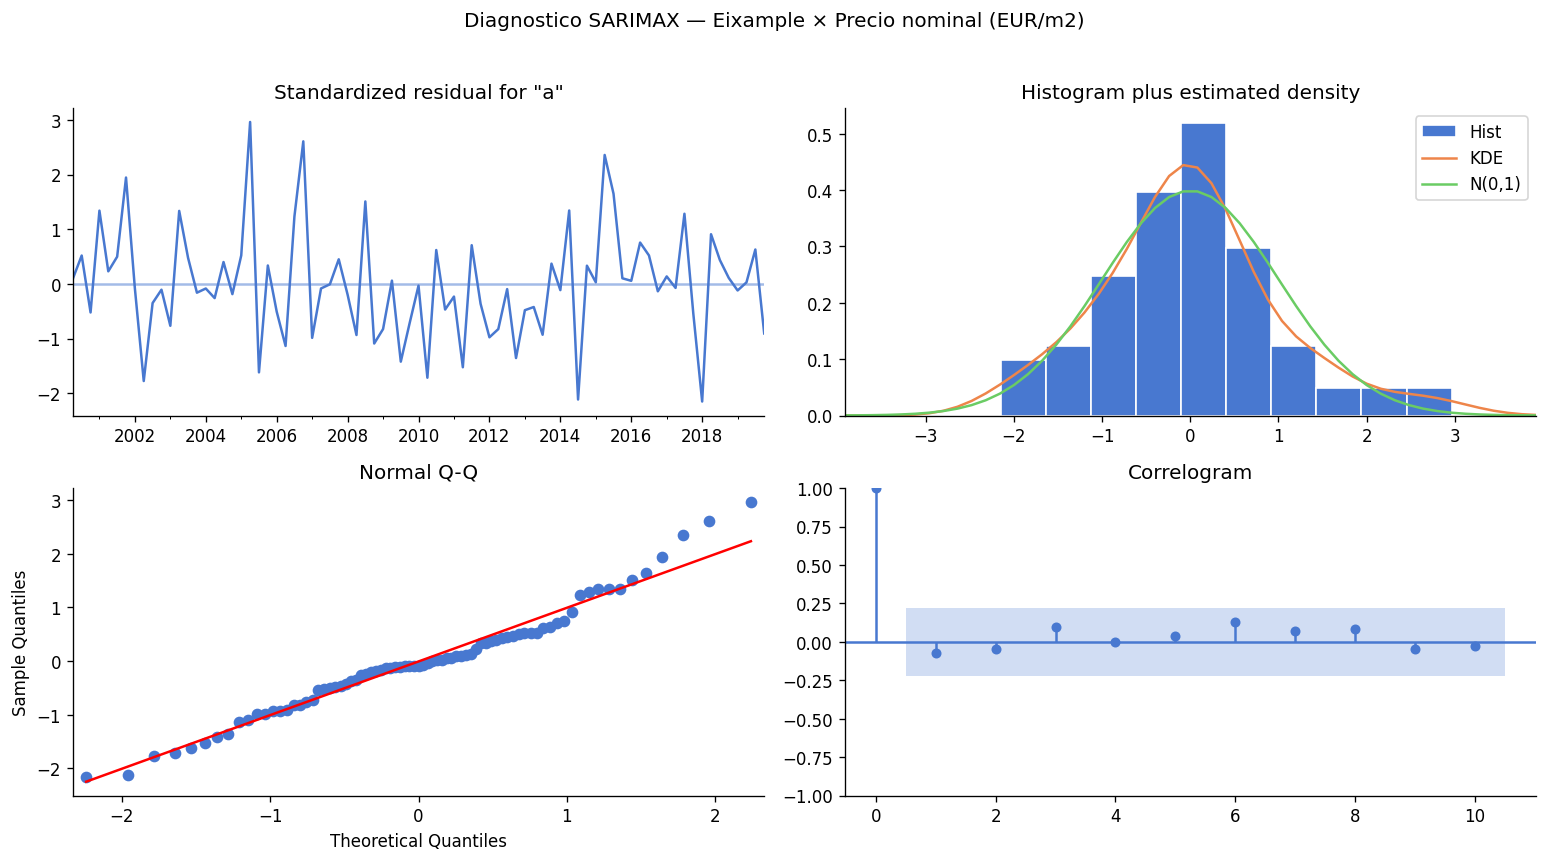
\includegraphics[width=\linewidth]{figures/fig09_diagnostics_sarimax.png}
  \caption{Diagnóstico SARIMAX, Eixample$\times$precio nominal. Cuatro paneles:
    residuos sin estructura temporal, distribución aproximadamente normal con
    colas ligeras, Q-Q con leve desviación en extremos, correlograma sin picos.
    Ljung-Box $p(8){=}0.985$ confirma ruido blanco.}
  \label{fig:diag}
\end{figure}

De las 30 combinaciones distrito$\times$métrica, solo Eixample$\times$contratos
rechaza la hipótesis nula de no-ARCH ($p{=}0.0007$). El resto confirma
homoscedasticidad y valida los intervalos de confianza del SARIMAX para precio
nominal y real en todos los distritos. Para Eixample$\times$contratos los IC
pueden estar subestimados;  para un futuro una posible mejora sería usar GARCH(1,1) para una inferencia más
precisa.

\subsection{Proyecciones condicionales y análisis de sustitución}

La Figura~\ref{fig:proj} muestra las proyecciones a 8 trimestres. Aplicando~\eqref{eq:indif}:
\begin{equation}
  \delta^* = \frac{1{,}588}{7{,}825} = 20.3\,\%
  \label{eq:indif_calc}
\end{equation}

\begin{figure}[!t]
  \centering
  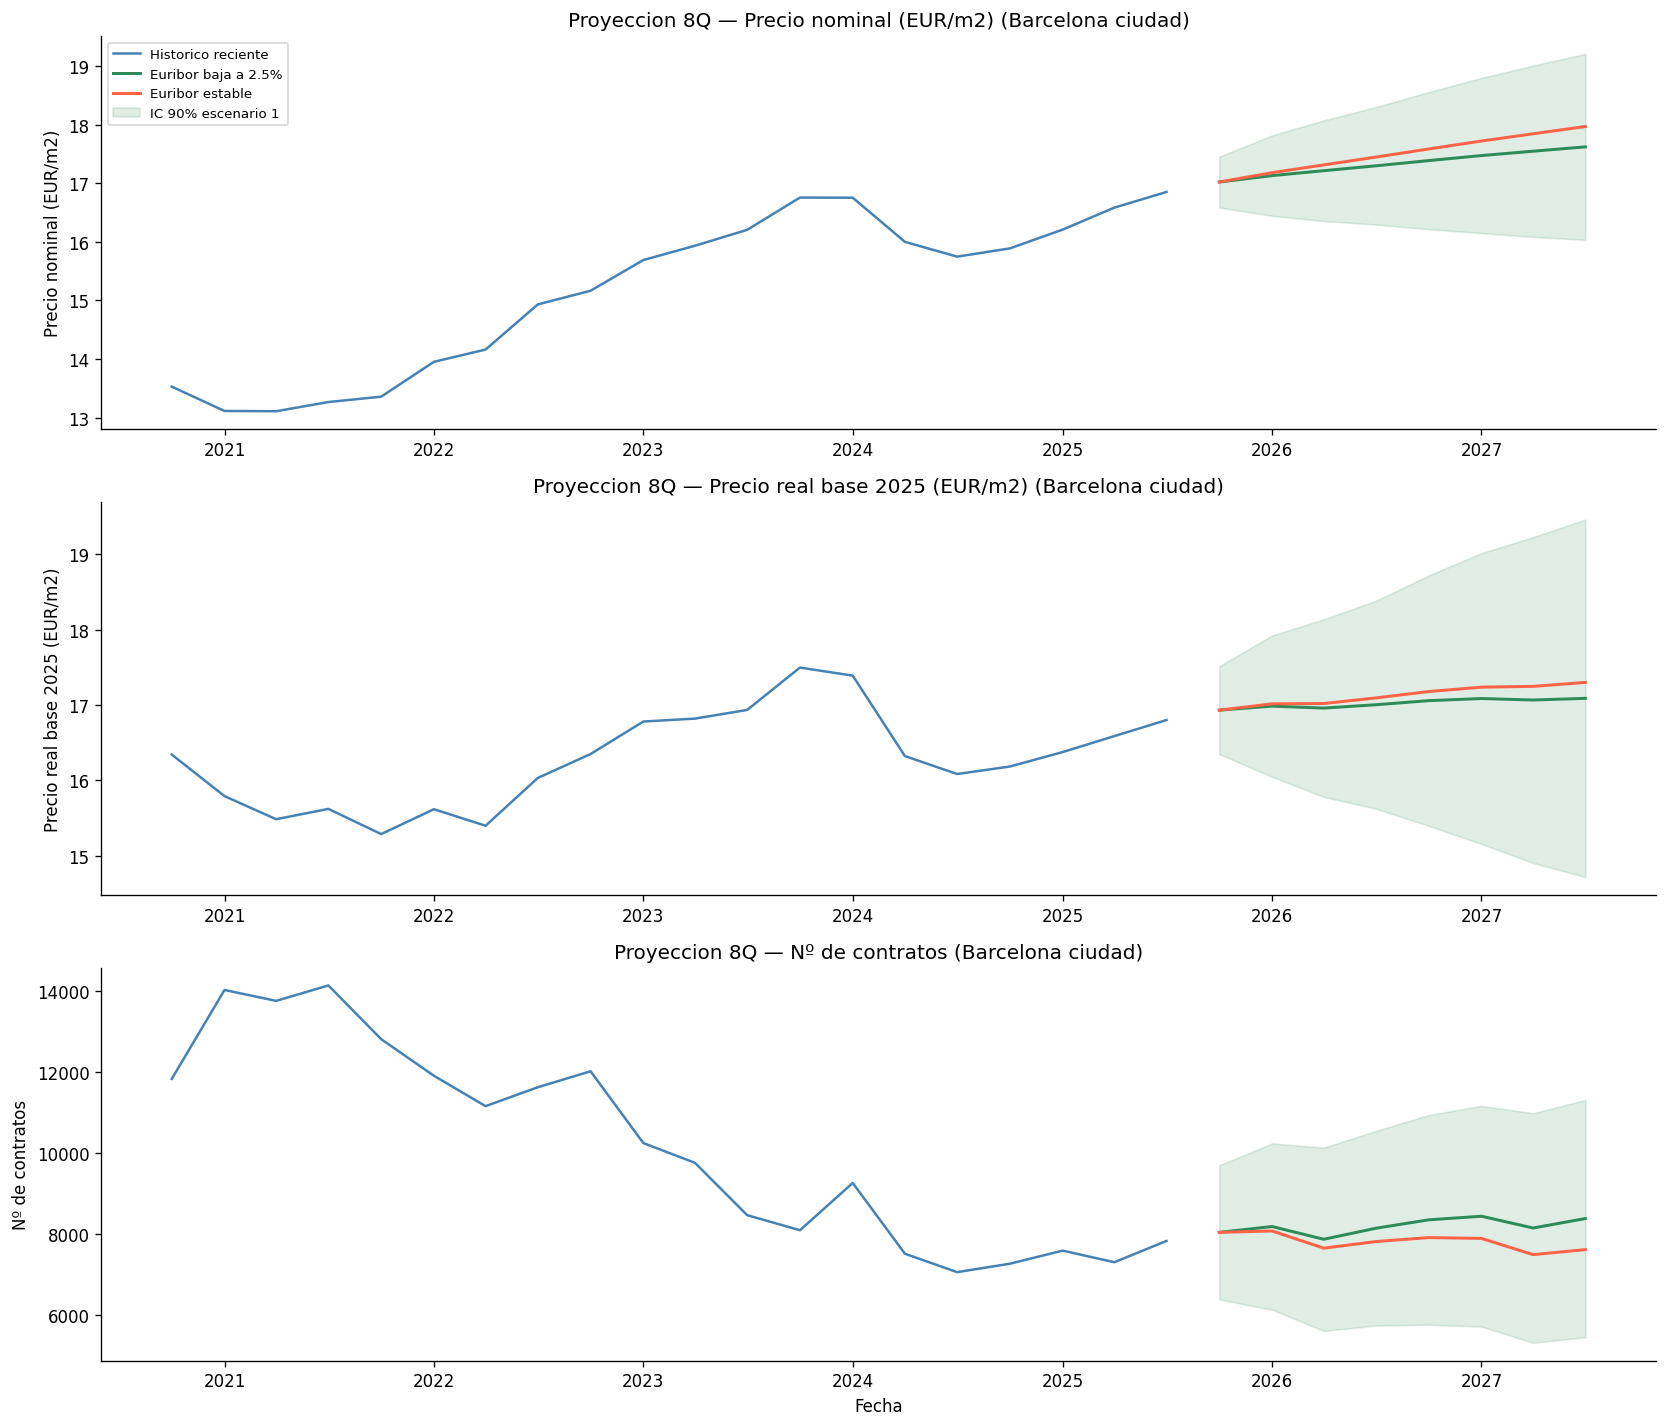
\includegraphics[width=\linewidth]{figures/fig08_projection.png}
  \caption{Proyecciones condicionales SARIMAX (8 trimestres, ciudad, 3 métricas).
    Verde: Euríbor baja de 2.12\,\% a 2.5\,\%. Rojo: Euríbor estable. Banda: IC\,90\,\%.
    Los dos escenarios convergen porque el ancla de 2.12\,\% ya está por debajo del
    2.5\,\% del escenario de bajada.}
  \label{fig:proj}
\end{figure}

La Figura~\ref{fig:proxy} visualiza la sensibilidad al sesgo de sustitución.

\begin{figure}[!t]
  \centering
  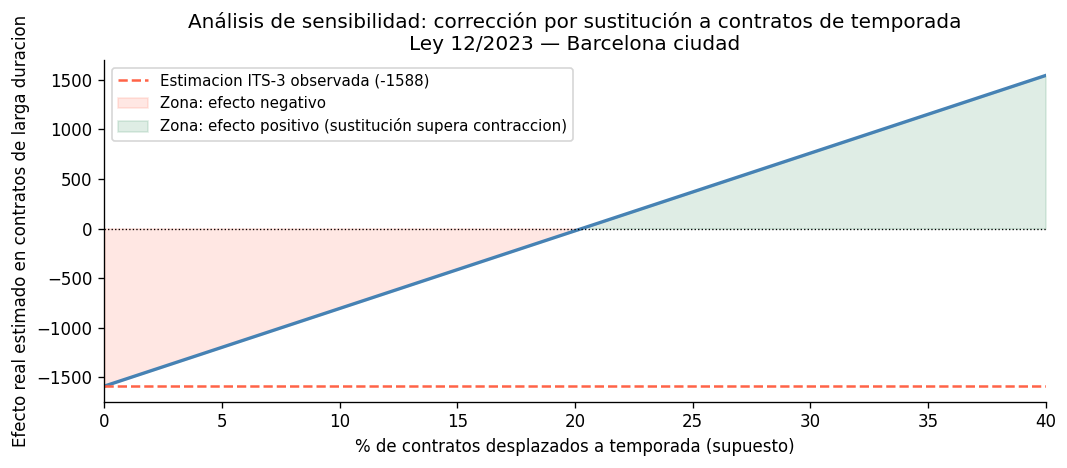
\includegraphics[width=\linewidth]{figures/fig11_substitution_proxy.png}
  \caption{Sensibilidad al sesgo de sustitución (Ley~12/2023). Eje $x$: porcentaje
    de contratos que hipotéticamente migraron a temporada. El punto de indiferencia
    (20.3\,\%) es la tasa crítica por encima de la cual el efecto real sobre volumen
    sería nulo. Zona roja: contracción neta robusta a la sustitución.}
  \label{fig:proxy}
\end{figure}

Bajo el escenario conservador (5\,\% de sustitución) el efecto real es $-1{,}197$
contratos/trimestre; bajo el moderado (15\,\%) es $-414$; el efecto se anularía
a partir del 20.3\,\%. Dado que las estimaciones de sustitución en la literatura
para Barcelona 2023--2025 oscilan entre el 15 y el 35\,\% \citep{bosch2021ley11},
el coeficiente negativo debe reportarse como cota superior de la contracción real
en el mercado de larga duración.

% ===========================================================
\section{Discusión}
\label{sec:discusion}

\subsection{El efecto composición como mecanismo dominante}

La paradoja precio-volumen, bajo la Ley~12/2023 --- reducción de $-1{,}588$
contratos por trimestre ($p{=}0.007$) simultánea a una subida de $+0.495$\,\euro/m$^2$
en precio real ($p{=}0.034$) --- no puede explicarse por un simple efecto de demanda.
El mecanismo más coherente es el efecto composición por retirada selectiva de oferta:
la regulación actúa como un filtro que expulsa del mercado de larga duración al stock
de menor calidad y precio (cuyo propietario no puede cubrir costes al precio regulado)
y retiene el stock de mayor calidad y precio (cuya renta regulada sigue siendo
atractiva frente al coste de oportunidad). La media ponderada $\bar{r}_t$ sube no
porque los precios individuales suban, sino porque la composición del stock
observable se desplaza hacia contratos de mayor valor unitario.

Este mecanismo es consistente con la no retroactividad de la ley: los contratos
vigentes antes de julio de 2023 quedaron excluidos de los topes de la Ley~12/2023,
de modo que el efecto inicial recae exclusivamente sobre el flujo de nuevos
contratos y renovaciones. Los propietarios con contratos de mayor precio relativo
tienen mayor incentivo a permanecer en el mercado habitual, lo que refuerza el
sesgo de composición al alza en los datos observados.

El modelo M5 confirma que esta retirada selectiva no es geográficamente discriminada:
el coeficiente de interacción $\hat\beta_{1a}{=}{-}0.019$ ($p{=}0.301$) indica que
el impacto sobre la actividad contractual es estadísticamente homogéneo entre barrios
de renta alta y baja en el estimador within. La heterogeneidad observada en el ITS-3
opera a nivel de magnitudes absolutas (Gràcia tiene mayor level shift que Nou Barris
porque su precio de partida es más alto), no a nivel de elasticidades relativas.

\subsection{La fase de transición regulatoria como período de anticipación}

El período P4 (vacío regulatorio, 2022Q2--2023Q2) muestra el efecto más claro en
precio real: $D_{tc}{=}{-}0.558$\,\euro/m$^2$ ($p{=}0.003$). Esta caída en precio
real durante el vacío regulatorio es contraintuitiva si se espera que la
desregulación permita subidas de precio; la explicación más plausible es que el
ajuste de contratos nuevos en el período de vacío se produjo principalmente en el
segmento nominal (donde sí hay subida), mientras que el deflactor IPC del período
2022--2023 fue excepcionalmente alto, reduciendo la métrica real de todos los
contratos del stock visible.

El período previo a la entrada en vigor de la Ley~12/2023 muestra señales de
comportamiento anticipatorio: propietarios con capacidad de gestión podrían haber
adelantado ajustes de renta, rotaciones de contrato o cambios a modalidad de
temporada antes de julio de 2023. Este efecto de anticipación haría que el level
shift $D_{ley12}$ recoja en parte el impacto de las decisiones tomadas antes de
la entrada en vigor legal, lo que tendería a amplificar el coeficiente estimado.
La distinción entre grandes tenedores y pequeños propietarios de la Ley~12/2023
es relevante aquí: los primeros tienen mayor capacidad de gestión estratégica y,
por tanto, mayor probabilidad de haber actuado anticipadamente.

\subsection{Las lag features como señal de inercia institucional}

El análisis SHAP revela que el retardo-4 del crecimiento de contratos
($\overline{|\phi_j|}{=}0.093$) supera a todas las variables de política
($\overline{|\phi_j|}{=}0.013$ para \texttt{post\_regulation}). Esto no invalida
el efecto regulatorio; lo contextualiza: la tensión contractual tiene inercia anual.
Un barrio que contrajo contratos en $t{-}4$ tiene alta probabilidad de seguir
haciéndolo en $t$, independientemente del régimen vigente. La implicación de
política es directa: la detección temprana de tensión requiere seguimiento
trimestral continuo, no indicadores anuales de referencia o señales instantáneas
de precio.

La interacción SHAP entre precio real y Euríbor muestra que en mercados asequibles
(precio real $< 14$\,\euro/m$^2$) la subida de tipos amplifica la probabilidad
de tensión. En mercados caros el efecto es más débil por el mayor buffer financiero
del perfil de inquilino. Este hallazgo apunta a que la política de ayuda al alquiler
que maximice la cobertura de episodios de tensión debería priorizar los segmentos
de menor precio real y mayor sensibilidad al Euríbor, no los segmentos de mayor
precio nominal visible.

\subsection{Validez del contrafactual ITS y limitaciones}

El contrafactual del ITS-3 descansa en tres supuestos documentados en la Sección
de metodología. El más comprometido en este diseño es el segundo: la ausencia de
confundidores simultáneos. El período 2020--2025 en Barcelona coincide con el
shock COVID, la crisis energética, el ciclo alcista del Euríbor y el boom del
turismo post-pandemia. Ninguno de estos factores tiene un instrumento de exclusión
perfecto dentro del modelo ITS-3; el Euríbor es el único controlado directamente
como exógena. Los resultados ITS y de panel son asociaciones parciales robustamente
estimadas, no efectos causales en sentido estricto.

La ausencia de grupo de control es la limitación central: todos los barrios de
Barcelona están bajo el mismo régimen regulatorio en cada período. Una extensión
con diferencias en diferencias usando municipios de la región metropolitana de
Barcelona como control mejoraría sustancialmente la identificación causal para
el período de la Ley~11/2020, donde existía variación geográfica en la aplicación.

% APLICAMOS BALANCE PARA IGUALAR LA ÚLTIMA PÁGINA ANTES DE TERMINAR
\balance 

% ===========================================================
\section{Conclusiones}
\label{sec:conclusiones}

\subsection{Respuestas a las tres preguntas de investigación}

Respondemos a continuación cada pregunta con los resultados más relevantes.

\textbf{RQ1 — Actividad contractual y regulación.} El estimador within de panel
asocia el período post-regulación con variaciones estadísticamente significativas
en la actividad contractual, condicionadas al Euríbor ($-0.076$, $p{<}.001$) y
al precio nominal ($-0.038$ por \euro/m$^2$, $p{<}.001$). M4 muestra que esta
asociación no es uniforme entre regímenes: la Ley~11/2020 tiene el coeficiente
más pronunciado y significativo ($+0.317$, $p{<}.001$), mientras que el vacío TC
y la Ley~12/2023 no son significativos en el within estimator. A nivel ciudad,
el SARIMAX con Euríbor reduce el MAPE a la mitad en precio nominal (3.29\,\%
vs.\ 6.97\,\% del naïve), confirmando que el canal de tipos de interés es la
principal fuerza macro explicativa de la trayectoria de precios.

\textbf{RQ2 — Localización y predicción de tensión.} Los lag features elevan el
AUC del Random Forest de 0.553 a 0.684 ($+0.131$), confirmado por validación
cruzada temporal ($0.684\pm0.083$). Los valores SHAP identifican el retardo anual
del crecimiento de contratos como señal dominante ($\overline{|\phi|}{=}0.093$),
superando a las variables de política. El panel logit con efectos fijos de barrio
complementa este resultado con coeficientes directamente interpretables que
conectan la probabilidad de tensión con los indicadores regulatorios del módulo
de panel. El techo de discriminación con las features disponibles se sitúa cerca
del 0.70, limitado por el shift distribucional entre los regímenes de entrenamiento
y test.

\textbf{RQ3 — Impacto de las intervenciones.} La Ley~11/2020 produce un level
shift inmediato de $-1.11$\,\euro/m$^2$ en precio nominal ($p{=}0.007$), sin
efecto en precio real. La derogación TC tiene el mayor impacto en precio real
($-0.558$\,\euro/m$^2$, $p{=}0.003$). La Ley~12/2023 contrae el volumen de
contratos de larga duración ($-1{,}588$/trimestre, $p{=}0.007$) y eleva
simultáneamente el precio real ($+0.495$\,\euro/m$^2$, $p{=}0.034$). Esta
paradoja precio-volumen es geográficamente consistente en los 9 de 10 distritos y
es cuantitativamente robusta al sesgo de sustitución hasta el 20.3\,\% de
migración a temporada.

\subsection{Líneas abiertas}

Cuatro extensiones serían de alto valor para trabajos futuros. Primero, incorporar
datos de contratos de temporada (duración $\leq 11$ meses) para estimar directamente
el flujo de sustitución y reducir la incertidumbre sobre el punto de indiferencia
$\delta^*$. Segundo, aplicar un diseño de diferencias en diferencias con municipios
metropolitanos u otras comunidades autónomas como control para el período Ley~11/2020, mejorando la identificación
causal. Tercero, aplicar GARCH(1,1) a Eixample$\times$contratos para calibrar
correctamente los intervalos de confianza predictivos en ese caso. Cuarto, extender
el panel logit a un modelo de panel probit con corrección de incidental parameters
para mitigar el sesgo de Neyman-Scott en muestras con muchos efectos fijos y horizonte
temporal moderado.

% ===========================================================
\bibliographystyle{apalike}
\begin{thebibliography}{99}

\bibitem[Angrist y Pischke, 2009]{angrist2009mostly}
Angrist, J.~D.\ y Pischke, J.-S. (2009).
\textit{Mostly Harmless Econometrics}.
Princeton University Press.

\bibitem[Antipov y Pokryshevskaya, 2020]{antipov2020shap}
Antipov, E.~A.\ y Pokryshevskaya, E.~B. (2020).
Interpretable machine learning for demand modeling with high-dimensional data.
\textit{Journal of Revenue and Pricing Management}, 19(2):90--97.

\bibitem[Arnott, 1995]{arnott1995rent}
Arnott, R. (1995).
Time for revisionism on rent control?
\textit{Journal of Economic Perspectives}, 9(1):99--120.

\bibitem[Baltagi, 2021]{baltagi2021econometric}
Baltagi, B.~H. (2021).
\textit{Econometric Analysis of Panel Data} (6.ª ed.).
Springer.

\bibitem[Bergmeir et~al., 2018]{bergmeir2018note}
Bergmeir, C., Hyndman, R.~J.\ y Koo, B. (2018).
A note on the validity of cross-validation for evaluating autoregressive time
series prediction.
\textit{Computational Statistics \& Data Analysis}, 120:70--83.

\bibitem[Bosch y Costa, 2021]{bosch2021ley11}
Bosch, J.\ y Costa, A. (2021).
Efectes de la Llei 11/2020 sobre el mercat de lloguer a Catalunya.
\textit{Papers -- Regió Metropolitana de Barcelona}, 63:12--25.

\bibitem[Box et~al., 2015]{box2015timeseries}
Box, G.~E.~P., Jenkins, G.~M., Reinsel, G.~C.\ y Ljung, G.~M. (2015).
\textit{Time Series Analysis: Forecasting and Control} (5.ª ed.).
Wiley.

\bibitem[Cruz et~al., 2019]{cruz2019its}
Cruz, M., Saá-Requejo, J.\ y Perpiñán, O. (2019).
Interrupted time series for policy evaluation with multiple interventions.
\textit{Statistics in Medicine}, 38(14):2605--2621.

\bibitem[Diamond et~al., 2019]{diamond2019rent}
Diamond, R., McQuade, T.\ y Qian, F. (2019).
The effects of rent control expansion on tenants, landlords, and inequality.
\textit{American Economic Review}, 109(9):3365--3394.

\bibitem[García-Montalvo y Raya, 2018]{garcia2018housing}
García-Montalvo, J.\ y Raya, J.~M. (2018).
Constraints on housing affordability in Spain.
\textit{Estudios sobre la Economía Española}, SERIEs.

\bibitem[Harvey, 1989]{harvey1989forecasting}
Harvey, A.~C. (1989).
\textit{Forecasting, Structural Time Series Models and the Kalman Filter}.
Cambridge University Press.

\bibitem[Hyndman y Athanasopoulos, 2021]{hyndman2021forecasting}
Hyndman, R.~J.\ y Athanasopoulos, G. (2021).
\textit{Forecasting: Principles and Practice} (3.ª ed.).
OTexts.

\bibitem[Kholodilin et~al., 2021]{kholodilin2021rent}
Kholodilin, K.~A., Kohl, S.\ y Pfeiffer, D. (2021).
Does rent control reduce rents? An economic analysis of Berlin's Mietendeckel.
\textit{DIW Berlin Discussion Paper}, 1927.

\bibitem[Lundberg y Lee, 2017]{lundberg2017shap}
Lundberg, S.~M.\ y Lee, S.-I. (2017).
A unified approach to interpreting model predictions.
\textit{Advances in Neural Information Processing Systems}, 30:4765--4774.

\bibitem[Molnar, 2020]{molnar2020interpretable}
Molnar, C. (2020).
\textit{Interpretable Machine Learning: A Guide for Making Black Box Models Explainable}.
Leanpub.

\bibitem[Módenes y López-Colás, 2021]{modenes2021alquiler}
Módenes, J.~A.\ y López-Colás, J. (2021).
El alquiler como modo de tenencia emergente en España.
\textit{Scripta Nova}, 25(660):1--22.

\bibitem[Newey y West, 1987]{newey1987hac}
Newey, W.~K.\ y West, K.~D. (1987).
A simple, positive semi-definite, heteroskedasticity and autocorrelation
consistent covariance matrix.
\textit{Econometrica}, 55(3):703--708.

\bibitem[Sims, 2007]{sims2007rent}
Sims, D.~P. (2007).
Out of control: what can we learn from the end of Massachusetts rent control?
\textit{Journal of Urban Economics}, 61(1):129--151.

\bibitem[Wagner et~al., 2002]{wagner2002its}
Wagner, A.~K., Soumerai, S.~B., Zhang, F.\ y Ross-Degnan, D. (2002).
Segmented regression analysis of interrupted time series studies.
\textit{Journal of Clinical Pharmacy and Therapeutics}, 27(4):299--309.

\bibitem[Incasol--Habitatge, 2025]{incasol2025}
{Incasol -- Generalitat de Catalunya / Habitatge} (2025).
Lloguers de Barcelona per districtes i barris.
\href{https://habitatge.gencat.cat/ca/dades/indicadors_estadistiques/estadistiques_de_construccio_i_mercat_immobiliari/mercat_de_lloguer/lloguers-barcelona-per-districtes-i-barris/}{Estadístiques de construcció i mercat immobiliari}.

\bibitem[INE, 2025]{ine2025ipc}
{Instituto Nacional de Estadística (INE)} (2025).
Índice de Precios de Consumo. Tabla 24078.
\href{https://www.ine.es/jaxiT3/Datos.htm?t=24078}{Series trimestrales, base~2025}.

\bibitem[Banco de España, 2025]{bde2025euribor}
{Banco de España} (2025).
Boletín Estadístico: Euríbor a 12 meses.
\href{https://app.bde.es/bie_www/bie_wwwias/xml/Arranque.html?Idioma=es}{Series mensuales}.

\bibitem[Idescat, 2025]{idescat2025ist}
{Institut d'Estadística de Catalunya (Idescat)} (2025).
Índice Socioeconómico Territorial (IST).
\href{https://www.idescat.cat/dades/obertes/ist/}{Dades obertes per barris}.

\end{thebibliography}
\usepackage{float}
% ---------------------------------------------------------
% En el documento:
\appendix

\section{Tablas de referencia}
\label{app:tablas}

\begin{table}[H]
\caption{Grid AIC/BIC SARIMAX (top 5 órdenes, Eixample$\times$nominal)}
\centering\small
\begin{tabular}{ccccrr}
\toprule
$p$ & $q$ & $P$ & $Q$ & AIC & BIC \\
\midrule
1 & 1 & 1 & 0 & \textbf{10.89} & 25.11 \\
2 & 1 & 1 & 0 & 12.05 & 28.64 \\
1 & 1 & 1 & 1 & 12.82 & 29.41 \\
1 & 1 & 0 & 1 & 12.94 & 27.15 \\
2 & 1 & 1 & 1 & 14.01 & 32.96 \\
\bottomrule
\end{tabular}
\end{table}

\noindent El orden $(1,1,1)(1,0,1)_4$ ocupa la posición~3 en AIC con
$\Delta\text{AIC}{=}1.93 < 2$ (intervalo de equivalencia estadística),
confirmando su validez metodológica frente al orden óptimo por AIC.

\begin{table}[H]
\caption{Distribución de market\_tension por año (barrios)}
\centering\small
\begin{tabular}{lrr}
\toprule
Año & N episodios & Tasa tensión (\%) \\
\midrule
2020 & -- & 68.6 \\
2021 & -- & 7.9  \\
2022 & -- & 54.3 \\
2023 & -- & 76.5 \\
2024 & -- & 61.9 \\
\bottomrule
\end{tabular}
\end{table}

\end{document}
